\documentclass[a4paper,11pt]{article}
	\usepackage[utf8]{inputenc}
	\usepackage[italian]{babel}
	\usepackage{hyperref}	%Consente l'inserimento di \url
	\usepackage{booktabs}	%Utilità di abbellimento tabelle
	\usepackage{longtable}
	\usepackage{tabularx}
	%\usepackage{widetable}
	\usepackage{array}
	\usepackage{listings}
	\usepackage{graphicx}
	\usepackage{caption}
	\usepackage{fancyhdr}
	\newenvironment{fixpic}{}{} % [1]
	\usepackage[a4paper,top=3cm,bottom=3cm,left=2.5cm,right=2.5cm]{geometry}
	%******
	\usepackage{makeidx}
	\usepackage{textcomp}
	\usepackage{multirow}
	\usepackage{rotfloat}
	\usepackage{lastpage}
	\usepackage{array}
	\usepackage{float}
	% *************************************
	% QUI CODICE PER \SUBSUBSUBSECTION
	\usepackage{titlesec}
	\titleclass{\subsubsubsection}{straight}[\subsection]
	
	\newcounter{subsubsubsection}[subsubsection]
	\renewcommand\thesubsubsubsection{\thesubsubsection.\arabic{subsubsubsection}}
	\renewcommand\theparagraph{\thesubsubsubsection.\arabic{paragraph}} % optional; useful if paragraphs are to be numbered
	
	\titleformat{\subsubsubsection}
	  {\normalfont\normalsize\bfseries}{\thesubsubsubsection}{1em}{}
	\titlespacing*{\subsubsubsection}
	{0pt}{3.25ex plus 1ex minus .2ex}{1.5ex plus .2ex}
	
	\makeatletter
	\renewcommand\paragraph{\@startsection{paragraph}{5}{\z@}%
	  {3.25ex \@plus1ex \@minus.2ex}%
	  {-1em}%
	  {\normalfont\normalsize\bfseries}}
	\renewcommand\subparagraph{\@startsection{subparagraph}{6}{\parindent}%
	  {3.25ex \@plus1ex \@minus .2ex}%
	  {-1em}%
	  {\normalfont\normalsize\bfseries}}
	\def\toclevel@subsubsubsection{4}
	\def\toclevel@paragraph{5}
	\def\toclevel@paragraph{6}
	\def\l@subsubsubsection{\@dottedtocline{4}{7em}{4em}}
	\def\l@paragraph{\@dottedtocline{5}{10em}{5em}}
	\def\l@subparagraph{\@dottedtocline{6}{14em}{6em}}
	\makeatother
	
	\setcounter{secnumdepth}{4}
	\setcounter{tocdepth}{4}
	%FINE \SUBSUBSUBSECTION
	%****************************************
	%STYLE PER INSERIMENTO DEL CODICE
	\lstdefinestyle{style1}{
	  belowcaptionskip=1\baselineskip,
	  breaklines=true,
	  frame=L,
	  xleftmargin=\parindent,
	  language=Pascal,
	  showstringspaces=false,
	  basicstyle=\footnotesize\ttfamily,
	  keywordstyle=\bfseries\color{blue},
	  commentstyle=\itshape\color{blue},
	  identifierstyle=\color{blue},
	  stringstyle=\color{orange},
	}
	
	\lstdefinestyle{style2}{
	  belowcaptionskip=1\baselineskip,
	  frame=L,
	  xleftmargin=\parindent,
	  language=C,
	  basicstyle=\footnotesize\ttfamily,
	  commentstyle=\itshape\color{blue},
	}
	\lstset{style=style1}
	
	%FINE STYLE INSERIMENTO CODICE
	%*****************************************
	\usepackage[default]{cantarell} %% Use option "defaultsans" to use cantarell as sans serif only
	\usepackage[T1]{fontenc}        %% for font
	\hypersetup{colorlinks, linkcolor=black, urlcolor=blue}
	\newcommand{\addglos}{\begin{scriptsize}{\textbf{\ped{G}}} \end{scriptsize}} 
	\pagestyle{fancy}
	\fancyhead{}
	\fancyfoot{}
	%\fancyhead[L]{
\includegraphics[scale=0.28]{team_not_found.jpeg}}
	\fancyhead[L]{
\includegraphics[scale=0.15]{../../team404_small.jpg} \hspace{2mm} QUIZZIPEDIA}
	\fancyhead[R]{\leftmark}
	\fancyfoot[L]{Universit\`a degli studi di Padova - IS 2015/2016 \\ \url{team404swe@gmail.com}}

	
	%Commando usato per la tabella di informazioni sul documento
	\newcommand{\introtab}[9]{
		\begin{table}[ht]
		\begin{center}		
		\begin{tabular}{r l}			
			\toprule		
			\multicolumn{2}{c}{\textbf{ Informazioni sul documento }} \\
			\midrule 
			\textbf{Nome Documento}			& \vline \hspace{3.5 mm} {#1} \\
			\textbf{Versione}				& \vline \hspace{3.5 mm} {#2} \\
			\textbf{Uso} 					& \vline \hspace{3.5 mm} {#3} \\
			\textbf{Data Creazione} 		& \vline \hspace{3.5 mm} {#4} \\
			\textbf{Data Ultima Modifica} 	& \vline \hspace{3.5 mm} {#5} \\
			\textbf{Redazione}				& \vline \hspace{3.5 mm} {#6} \\
											%& \vline \hspace{3.5 mm} {#7} \\	
			\textbf{Verifica} 				& \vline \hspace{3.5 mm} {#7}	\\
			\textbf{Approvazione}			& \vline \hspace{3.5 mm} {#8}\\	
			\textbf{Committente} 			& \vline \hspace{3.5 mm} Zucchetti SPA\\
			\textbf{Lista di distribuzione} & \vline \hspace{3.5 mm} Prof. Vardanega Tullio \\														& \vline \hspace{3.5 mm} TEAM404 \\
	\bottomrule	
	\end{tabular}
	\end{center}
	\end{table}
	}
	% Comando di inizio del registro
	\newcommand{\beginregistro}{
		%\begin{longtable}{{|p{0.10\textwidth}|p{0.20\textwidth}|p{0.15\textwidth}|p{0.50\textwidth}|}}
		\begin{longtable}{{|p{1.5cm}|p{2.5cm}|p{2cm}|p{8cm}|}} 
	 		\hline	
	}
	% commando usato pr inserire una riga al registro delle modifiche
	\newcommand{\rigaregistro}[4]{
		{\footnotesize #1} & {\footnotesize #2} &  {\footnotesize #3} &  {\footnotesize #4} \\
			\hline	
	}
	% Comando di fine registro
	\newcommand{\fineregistro}{ \end{longtable}	}
	
	%************************************************
	% commandi per il GLOSSARIO
	%***********************************************
	% Commando di inizio tabella Glossario
	\newcommand{\beginglos}{
		\begin{longtable}{{p{0.20\textwidth}p{0.65\textwidth}}}	
	}
	% Commando per i termini del glossario
	
	\newcommand{\itemglos}[2]{
		\textbf{#1 :} & {#2} \\ \\ \\
	}
	% Commando fine Glossario
	\newcommand{\fineglos}{ \end{longtable} }
	% Comando per aggiungere una ssezione numerata con lettere al glossario
	\newcommand{\sezione}{
	\subsection{}	
	\rule[0.3pt]{\linewidth}{0.4pt} \\ % Linea orizzontale
	}
	
\newcommand{\sezioneglos}[1] { 
  \newpage
  \cleardoublepage
  \phantomsection
  \addcontentsline{toc}{section}{#1}
  \vspace{11pt}
  \textbf{\huge{#1} } % Lettera grande 
  \\
  \rule[0.3pt]{\linewidth}{0.4pt} \\ % Linea orizzontale
  \fancyhead[R]{#1}
}
\usepackage[utf8]{inputenc}
\usepackage{hyperref}	%Consente l'inserimento di \url
\usepackage{booktabs}	%Utilità di abbellimento tabelle
\usepackage{caption}	%Caption tabelle
\usepackage{graphicx}   %Inserimento immagini
\usepackage{tabularx}	%tabelle migliorate
\usepackage{eurosym}	%Inserimento del simbolo €
\usepackage{geometry}	%Spostamento di elementi nella pagina
\usepackage{color}		%Cambiare colore al font
\usepackage{fancyref}	%riferimenti più strutturati
\hypersetup{colorlinks, linkcolor=black, urlcolor=blue}


\graphicspath{ {./Images/} }
\title{\textbf{{\fontsize{10mm}{6mm}\selectfont QUIZZIPEDIA}}}

\makeindex

\begin{document}
	\maketitle
	
	\begin{center}

	
\includegraphics{../../team_not_found.jpg}\\	
	\fontsize{5mm}{3mm}\url{team404swe@gmail.com}\\
	\vspace{40mm}
	\textbf{ Piano di Progetto 3.0}
	\end{center}
	\thispagestyle{empty}	% per togliere il numero in fondo pagina
	\introtab{Piano di Progetto}			%1 nome documento
			{3.0} 							%2 versione
			{Esterno} 						%3 Uso
			{21 dicembre 2015} 				%4 Data cre
			{\today} 						%5 Data mod
			{D. Bortot - M. Mbouenda}		%6 Redazione1
			%{} 							%7 Redazione2
			{Andrea Multineddu} 			%8 Verifica
			{Alex Beccaro} 				%9 Approvazione
	
	\newpage
	\thispagestyle{empty}
	\null
	
	\newpage
	\fancyfoot[R]{\thepage}
	\pagenumbering{Roman}
	\section*{Registro delle modifiche}
		\begin{longtable}{{|p{0.10\textwidth}|p{0.15\textwidth}|p{0.15\textwidth}|p{0.50\textwidth}|}} 
	 		\hline			
\rigaregistro{\textbf{Versione}}{\textbf{Autore}}{\textbf{Data}}						{\hspace{5 mm} \textbf{Descrizione}}	
			
			\rigaregistro{3.0}{A. Beccaro   \newline(Responsabile)}{12/06/2016}{Approvazione documento. }
			\rigaregistro{2.2}{M. Mbouenda  \newline(Verificatore)}{12/06/2016}{ verificate le sezioni §\ref{con:consuper} e \ref{con:prevfinire}}
			\rigaregistro{2.1.3}{A. Beccaro  \newline(Responsabile)}{02/06/2016}{aggiunta preventivo a finire \ref{con:prevfinire} }
			\rigaregistro{2.1.2}{A. Beccaro  \newline(Responsabile)}{01/06/2016}{aggiunta consuntivo di periodo in §\ref{con:consuper} }
			\rigaregistro{2.1.1}{M. Crivellaro  \newline(Responsabile)}{30/05/2016}{aggiunta Fase di Progettazione di dettaglio e codifica in sezione §\ref{conto:consuntivo}}			
			\rigaregistro{2.1.0}{A. Multineddu  \newline(Verificatore)}{29/05/2016}{Verifica della sezione §\ref{risk:rischi} e delle sotto sezioni §\ref{risk:risorse}, §\ref{risk:conoscenze }, §\ref{risk: errori} ,§\ref{risk:ritardi } }
			\rigaregistro{2.0.3}{M. Crivellaro  \newline(Responsabile)}{28/05/2016}{completamento analisi dei rischi in §\ref{risk:risorse}, §\ref{risk:conoscenze }, §\ref{risk: errori} ,§\ref{risk:ritardi } }
			\rigaregistro{2.0.2}{M. Crivellaro \newline(Responsabile)}{28/05/2016}{inizio analizzi dei rischi per la fase di progettazione di dettaglio e codifica.}
			\rigaregistro{2.0.1}{M. Crivellaro \newline(Responsabile)}{27/05/2016}{modifica di 'Analisi Dinamica' in 'Riscontro'.}
			
					
			\rigaregistro{2.0}{M. Mbouenda \newline(Verificatore)}{12/05/2016}{Approvazione documento.}
			\rigaregistro{1.3}{A. Multineddu \newline(Verificatore)}{12/05/2016}{Correzioni tabelle sezione §8.2.x.}
			\rigaregistro{1.2.1}{M. Mbouenda \newline(Responsabile)}{11/05/2016}{Correzioni tabelle sezione §8.2.x.}
			\rigaregistro{1.2}{A. Beccaro \newline(Verificatore)}{10/05/2016}{Verifica sottosezione §8.2.x: rivedere tabelle  .}
			\rigaregistro{1.1.2}{M. Mbouenda \newline(Responsabile)}{07/05/2016}{Definizione e stesura sottosezioni §8.2.2.1, §8.2.2.2, §8.2.2.3 .}
			\rigaregistro{1.1.1}{M. Mbouenda \newline(Responsabile)}{05/05/2016}{Definizione sottosezioni §8.2, §8.2.1, §8.2.2 .}
			\rigaregistro{1.1}{A. Beccaro \newline(Verificatore)}{04/05/2016}{Verificate le modifiche della versione 1.0.x del documento.}
			\rigaregistro{1.0.6}{D. Bortot \newline(Responsabile)}{02/05/2016}{Aggiunte considerazioni finali in §8.1.2.4}
			\rigaregistro{1.0.5}{D. Bortot \newline(Responsabile)}{01/05/2016}{Inserita corretta nomenclatura del verbale in §8.1.1. Aggiornata versione dei documenti di riferimento in §2.2 e §2.3}
			\rigaregistro{1.0.4}{D. Bortot \newline(Responsabile)}{29/04/2016}{Definite le sezioni §8.1.2.2, §8.1.2.3 e la sezione "Preventivo" §8.1.2.4 con le relative tabelle.}
			\rigaregistro{1.0.3}{D. Bortot \newline(Responsabile)}{26/04/2016}{Definita la sezione §8.1.1, prima stesura di §8.1.2, generate le tabelle e il grafico di §8.1.2.1}	
			\rigaregistro{1.0.2}{D. Bortot \newline(Responsabile)}{24/04/2016}{Introdotta la parte di analisi dinamica dei rischi. Modificato l'impianto del capitolo §5, ora ogni rischio comprende anche gli elementi: 'Controllo','Gestione' e 'Analisi Dinamica'. Modificati di conseguenza l'introduzione di "Analisi dei rischi" e la specifica di ogni rischio (per ora comprendendo solo il periodo "Analisi iniziale" in 'Analisi dinamica'). Integrati i contenuti di §5.5 in  §5.4.1.}
			\rigaregistro{1.0.1}{D. Bortot \newline(Responsabile)}{23/04/2016}{Prima stesura del capitolo §8, "Consuntivi". Definita la sezione §8.1, generato grafico e tabella.}
			\rigaregistro{1.0}{D. Bortot \newline(Responsabile)}{06/04/2016}{Approvazione documento.}
			\rigaregistro{0.4}{A. Multineddu \newline(Verificatore)}{05/04/2016}{Revisione sezioni modificate.}
			\rigaregistro{0.3.2}{D. Bortot \newline(Responsabile)}{04/04/2016}{Aggiunta la scelta "RP-max" alla sezione 6.2.3. Aggiunte valutazioni sul costo dell'analisi iniziale in 7.2. Aggiunta la sezione 5.5 "Controllo dei rischi" e la Figura 1.}
			\rigaregistro{0.3.1}{D. Bortot \newline(Responsabile)}{29/03/2016}{Eliminata ridondanza di definizione dei Ruoli di Progetto, con conseguente ristesura della sezione 3.2.}
			\rigaregistro{0.3}{A. Multineddu \newline(Verificatore)}{15/03/2016}{Revisione totale.}
			\rigaregistro{0.2.1}{D. Bortot \newline(Responsabile)}{14/03/2016}{Aggiustamenti minori alla formattazione del documento, correzione typo.}
			\rigaregistro{0.2}{A. Luca \newline(Verificatore)}{14/03/2016}{Revisione di stile. Segnalazione errori tipografici.}
			\rigaregistro{0.1.2}{D. Bortot \newline(Responsabile)}{06/03/2016}{Aggiustamento  dei capitoli 6 e 7, rivalutati su un preventivo minimo adeguato al gruppo da 6 elementi.}
			\rigaregistro{0.1.1}{D. Bortot \newline(Responsabile)}{22/01/2016}{Aggiustamento sezione 2.2}
			\rigaregistro{0.1}{A. Multineddu \newline(Verificatore)}{22/01/2016}{Prima revisione del documento, segnalato errore nella sezione 2.2}
			\rigaregistro{0.0.5}{D. Bortot \newline(Responsabile)}{18/01/2016}{Generazione e inserimento dei grafici relativi ai capitoli 6 e 7, e completamento di quest'ultimi.}
			\rigaregistro{0.0.4}{D. Bortot \newline(Responsabile)}{08/01/2016}{Completamento di testo e tabelle della "Pianificazione". Prima stesura del "Conto Economico Preventivo".}
			\rigaregistro{0.0.3}{D. Bortot \newline(Responsabile)}{03/01/2016}{Completamento "Analisi dei rischi". Primo abbozzo di "Pianificazione".}
			\rigaregistro{0.0.2}{D. Bortot \newline(Responsabile)}{28/12/2015}{Completamento "Introduzione". Redazione dei capitoli "Organizzazione" e "Analisi del ciclo di vita software". Primo abbozzo dell' "Analisi dei rischi".}
			\rigaregistro{0.0.1}{D. Bortot \newline(Responsabile)}{21/12/2015}{Prima stesura del documento. Prima redazione del paragrafo "Introduzione".}		
			\caption{Versionamento del documento} 
		\end{longtable}
		
	\newpage
	\tableofcontents
	
	\newpage
	\listoftables
	\listoffigures	
	
	\newpage
	\pagenumbering{arabic}
	\section{Sommario}
	Questo documento illustra il Piano di Progetto del gruppo \textbf{Team404} relativo al capitolato \textbf{Quizzipedia}, commissionato da \textbf{Zucchetti S.p.A.}
	\\
	Lo scopo del documento è definire e presentare al committente le scelte progettuali significative adottate (quali il modello di ciclo di vita scelto per lo sviluppo e la politica di gestione dei rischi adottata), le problematiche d'interesse incontrate durante l'avanzamento ed un'adeguata offerta tecnico-economica relativa al progetto.
	
	\newpage
	\section{Introduzione}
	\subsection{Scopo del documento}
	Nelle sezioni successive del presente documento, dopo una rapida visione d'insieme del prodotto che il gruppo \textbf{Team404} si prefigge di sviluppare, verrà presentato l'organigramma del gruppo e la definizione dei ruoli di progetto, relativa assegnazione dei ruoli e la pianificazione delle risorse , l'analisi dei rischi correlata ed il piano economico preventivo.
	\subsection{Scopo del prodotto}
	Il progetto \textbf{Quizzipedia} ha come obiettivo lo sviluppo di un sistema software basato su tecnologie Web (Javascript\addglos, Node.js\addglos, HTML5\addglos, CSS3\addglos) che permetta la creazione, gestione e fruizione di questionari. Il sistema dovrà quindi poter archiviare i questionari suddivisi per argomento, le cui domande dovranno essere raccolte attraverso uno specifico linguaggio di markup (Quiz Markup Language) d'ora in poi denominato QML\addglos. In un caso d'uso a titolo esemplificativo, un "esaminatore" dovrà poter costruire il proprio questionario scegliendo tra le domande archiviate, ed il questionario così composto sarà presentato e fruibile all' "esaminando", traducendo l'oggetto QML\addglos in una pagina HTML\addglos, tramite un'apposita interfaccia web. Il sistema presentato dovrà inoltre poter proporre questionari preconfezionati e valutare le risposte fornite dall'utente finale.
	\\
	Per un'analisi più approfondita del progetto si rimanda al documento "\textit{analisi\_dei\_requisiti\_3.0.pdf}".
	\subsection{Glossario}
	Viene allegato un glossario nel file ``\textit{glossario\_3.0.pdf}'' nel quale viene data una definizione a tutti i termini che in questo documento appaiono con il simbolo "\addglos" a pedice .
	\subsection{Riferimenti}
		\subsubsection{Normativi}
		\begin{itemize}
			\item Capitolato d'appalto Quizzipedia:\\
			\url{http://www.math.unipd.it/~tullio/IS-1/2015/Progetto/C5.pdf}
			\item Norme di Progetto: "\textit{norme\_di\_progetto\_3.0.pdf}"
		\end{itemize}
		\subsubsection{Informativi}
		\begin{itemize}
			\item Corso di Ingegneria del Software anno 2015/2016:\\
			\url{http://www.math.unipd.it/~tullio/IS-1/2015/}
			\item Regole del progetto didattico:\\
			\url{http://www.math.unipd.it/~tullio/IS-1/2015/Dispense/PD01.pdf}
			\url{http://www.math.unipd.it/~tullio/IS-1/2015/Progetto/}\\
			\url{http://www.math.unipd.it/~tullio/IS-1/2015/Progetto/PD01b.html}
		\end{itemize}
	\pagebreak
	
	\newpage
	\section{Organizzazione}	
	\subsection{Organigramma}
	\subsection*{Redazione}
	\begin{table}[h!]
		\begin{tabularx}{\textwidth}{XcX}
			\textbf{Nominativo} & \textbf{Data} &\hspace{20 mm}  \textbf{Firma}\\
			\midrule
			Davide Bortot & 18/01/2016 & \hspace{20 mm} 
\includegraphics[scale=0.35]{../Firme/db.jpg} \\
			\midrule
		\end{tabularx}
	\caption{Redazione documento}
	\end{table}

	\subsection*{Revisione}
	\begin{table}[h!]
		\begin{tabularx}{\textwidth}{XcX}
			\textbf{Nominativo} & \textbf{Data} &\hspace{20 mm}  \textbf{Firma}\\
			\midrule
			Andrea Multineddu & 15/03/2016 & \hspace{20 mm} 
\includegraphics[scale=0.3]{../Firme/multi.jpg} \\
			\bottomrule
		\end{tabularx}
	\caption{Revisione documento}
	\end{table}
	
	\subsection*{Approvazione}
	\begin{table}[h!]
		\begin{tabularx}{\textwidth}{XcX}
			\textbf{Nominativo} & \textbf{Data} &\hspace{20 mm}  \textbf{Firma}\\
			\midrule
			Davide Bortot & 15/03/2016 & \hspace{20 mm} 
\includegraphics[scale=0.35]{../Firme/db.jpg} \\ 
			\bottomrule
		\end{tabularx}
	\caption{Approvazione documento}
	\end{table}

	\subsection*{Accettazione dei componenti}
	\begin{table}[h!]
		\begin{tabularx}{\textwidth}{XcX}
			\textbf{Nominativo} & \textbf{Data} &\hspace{20 mm}  \textbf{Firma}\\
			\midrule
			Davide Bortot & 18/01/2016 & \hspace{20 mm} 
\includegraphics[scale=0.3]{../Firme/db.jpg}\\	
				Martin Vadice Mbouenda & 08/03/2016 & \hspace{20 mm} 
\includegraphics[scale=0.35]{../Firme/martin.png} \\ 
				Marco Crivellaro & 10/03/2016 &\hspace{20 mm} 
\includegraphics[scale=0.3]{../Firme/crivellaro.png} \\ 
				Alex Beccaro & 08/03/2016 & \hspace{20 mm} 
\includegraphics[scale=0.3]{../Firme/becks.jpg} \\ 
				Luca Alessio & 10/03/2016 & \hspace{20 mm} 
\includegraphics[scale=0.3]{../Firme/alessio.jpg} \\ 
				Andrea Multineddu & 10/03/2016 & \hspace{20 mm} 
\includegraphics[scale=0.3]{../Firme/multi.jpg} \\ 
			\bottomrule
		\end{tabularx}
	\caption{Accettazione dei componenti}
	\end{table}
		\newpage
	\subsubsection*{Componenti}
			\begin{table}[h!]			
				\begin{center}
				\begin{tabular}{l c l}
				\textbf{Nominativo} & \textbf{Matricola} & \textbf{Posta elettronica}\\
				\midrule
				Davide Bortot & 1070213 & davide.bortot94@gmail.com \\
				Martin Vadice Mbouenda & 601901 & tinovad@hotmail.com \\
				Marco Crivellaro & 544339 & marcocrivellaro0603@gmail.com \\
				Alex Beccaro & 1072686 & alex.becks@hotmail.it \\
				Luca Alessio & 1070690 & lucaalessio1994@gmail.com \\
				Andrea Multineddu & 1049261 & andrea.multineddu@gmail.com \\
				\midrule
				\end{tabular}
			\end{center}
			\caption{Componenti}
			\end{table}	

	\subsection{Ruoli di progetto}
		Per un più sistematico sviluppo di progetto, e per adempiere alle regole di progetto riportate nella sezione Riferimenti, ai componenti del gruppo verranno assegnati nel tempo 6 diversi ruoli: \textbf{Responsabile}, \textbf{Amministratore}, \textbf{Analista}, \textbf{Progettista}, \textbf{Programmatore} e \textbf{Verificatore} la cui definizione è data nel documento "\textit{norme\_di\_progetto\_3.0.pdf}". La pianificazione delle risorse assicurerà che tutti gli elementi del gruppo ricopriranno almeno una volta ognuno dei ruoli riportati, in modo da poter spaziare nei vari ambiti dello sviluppo software.
		
	\pagebreak	
	
	\newpage
	\section{Analisi del ciclo di vita software}	
	In questo capitolo vengono presentati i principali modelli di ciclo di vita applicabili allo sviluppo del progetto software in questione, e viene in seguito spiegata la scelta del modello che il gruppo \textbf{Team404} ha deciso di adottare per \textbf{Quizzipedia}.
	\subsection{Modelli di cicli di vita}
	Segue la descrizione dei modelli attinenti alla scelta del gruppo; una panoramica di questi ed altri modelli di ciclo di vita del software è reperibile all'indirizzo: 
	
	"\url{http://www.math.unipd.it/~tullio/IS-1/2015/Dispense/L03.pdf}".
	\subsubsection{Modello Iterativo}
	I modelli iterativi prevedono che lo sviluppo proceda in fasi sequenziali e ben distinte da condizioni d'entrata e d'uscita, ammettendo però che errori ed imprevisti nel percorso (quale la variazione dei requisiti del sistema) riportino lo sviluppo ad uno stadio precedente per applicare le correzioni/migliorie necessarie. Queste caratteristiche rendono il modello adatto a progetti in cui errori di progettazione e analisi, o variazioni dei requisiti, sono molto probabili, consentendo di mantenere maggior parte del lavoro fatto e di ripartire prontamente da uno stato d'integrità noto del sistema. Come s'intuisce il modello non ha però sicurezza di convergenza, e rischia quindi di estendere negativamente i tempi di sviluppo.
	\subsubsection{Modello Incrementale}
	Il modello incrementale è un raffinamento del modello iterativo. Lo sviluppo procede per rilasci multipli e successivi, ciascuno dei quali realizza un incremento di funzionalità. L'analisi dei requisiti e la progettazione architetturale vengono eseguite solamente una volta all'inizio, identificando e fissando così univocamente i requisiti di base del progetto. Si avanza poi tramite cicli incrementali, procedendo a soddisfare prima i requisiti essenziali, e poi quelli opzionali e desiderabili. Ogni ciclo viene decomposto in:
	\begin{enumerate}
	\item Sviluppo dell'incremento di sistema;
	\item Validazione dell'incremento;
	\item Integrazione dell'incremento;
	\item Validazione del sistema.
	\end{enumerate}
	Così facendo alla fine di ogni ciclo il sistema è sempre in uno stato consistente, ed ogni incremento aggiunge valore al sistema. Il modello incrementale è quindi adatto a progetti in cui i requisiti fondamentali sono ben definiti, così da formare una solida struttura di base alla quale aggiungere incrementalmente funzionalità.

	\subsection{Scelta del modello}
	Il modello di ciclo di sviluppo (non sarà un ciclo di vita, mancando la parte di manutenzione) scelto per \textbf{Quizzipedia} è il modello Incrementale; essendo infatti il capitolato d'appalto ben strutturato e i requisiti essenziali ben specificati, è ragionevole definire nelle prime fasi del progetto una struttura di base alla quale aggiungere incrementalmente funzionalità nei momenti successivi dello sviluppo. Il modello adottato inoltre garantisce una decente convergenza e un avanzamento continuo, riducendo il rischio di ritardi di consegna, o peggio ancora la mancata partecipazione ad una revisione.
Altri modelli possibili sono stati scartati per le seguenti motivazioni:
	\begin{itemize}
		\item \textbf{Modello Iterativo}: è la versione meno controllata, e di conseguenza più soggetta ad errori, del modello incrementale;
		\item\textbf{Modello a Spirale}: applicabile soprattutto a progetti che devono rispondere spesso e prontamente a rischi particolarmente impattanti. Non è il caso di questo progetto;
		\item\textbf{Modello Evolutivo}: adatto a rispondere bisogni inizialmente non preventivabili, tramite più versioni di sviluppo parallele. Eccessivamente dispendioso per il progetto in questione.
	\end{itemize}
	
	\newpage
	
	\section{Analisi dei rischi} \label{risk:rischi}
	In questo capitolo verranno valutati i rischi e gli impedimenti che possono insorgere durante l'intera durata dello sviluppo del progetto. Per meglio strutturare e comprendere il problema a ogni rischio verranno associate:
	\begin{itemize}
	\item \textbf{Descrizione:} descrizione testuale del problema in analisi.
	\item \textbf{Probabilità:} una stima probabilistica che il problema si presenti, valutata in una scala da 1 a 3, dove 3 è il massimo.
	\item \textbf{Impatto:} l'influenza negativa che avrebbe il presentarsi del problema in analisi, valutato con una scala a tre livelli (A, B, C) dove:
		\begin{itemize}
			\item \textbf{A)} problema poco impattante e facilmente risolvibile;
			\item \textbf{B)} problema impattante ma risolvibile con soluzioni adeguate;
			\item \textbf{C)} problema molto impattante e difficilmente risolvibile.
		\end{itemize}
	\item \textbf{Controllo:} le tecniche da attuare per tenere sotto controllo il livello del rischio;
	\item \textbf{Gestione:} verrà suggerita per ogni rischio una strategia indicata a ridurne l'impatto, ove possibile;
	\item \textbf{Riscontro:} per ogni periodo di progetto viene riportato se il rischio si è presentato e se la gestione attuata si è dimostrata efficace. 
	\end{itemize}
	
	\subsection{Risorse Umane} \label{risk:risorse}
		\subsubsection{Incompatibilità componenti del gruppo}
		Rappresenta la possibilità che tra i componenti del gruppo sorgano incongruenze tali da impedire il corretto avanzamento del progetto.
		\begin{itemize}
		\item \textbf{Probabilità:} 1
		\item \textbf{Impatto:} B
		\item \textbf{Controllo:} sarà compito del Responsabile assicurare la corretta comunicazione tra i componenti e monitorare le problematiche.
		\item \textbf{Gestione:} nel caso il problema si verificasse sarà necessario l'intervento di un'autorità maggiore (prima fra tutte il Responsabile di progetto) che appiani le divergenze. Nel caso le controversie persistano è valutabile l'opzione di estromettere dal gruppo l'elemento più problematico;
		\item \textbf{Riscontro:}
			\begin{itemize}
				\item\textbf{Analisi Iniziale:} il rischio non si è presentato.
				\item\textbf{Progettazione:} il rischio non si è presentato. Fino al momento della stesura del presente documento, il gruppo è stato coeso e propenso a trovare facilmente strategie e idee di comune accordo.
				\item\textbf{Progettazione di dettaglio e codifica:} il rischio non si è presentato. 
			\end{itemize}
		\end{itemize}
		\subsubsection{Impegni esterni al progetto didattico}
		Rappresenta la possibilità che alcuni elementi del gruppo non riescano ad adempiere ai propri doveri progettuali a causa di impegni personali o universitari.
		\begin{itemize}
		\item \textbf{Probabilità:} 2
		\item \textbf{Impatto:} B
		\item \textbf{Controllo:} questo tipo di problema è stimabile ed evitabile fin dall'inizio del progetto tramite una dichiarazione, anche informale, dei propri obiettivi ed impegni da parte di tutti i componenti del gruppo. Così facendo si possono adeguatamente preventivare le ore di lavoro necessarie venendo incontro ad alle esigenze personali.
		\item \textbf{Gestione:} nel caso di eventi/impegni inaspettati la scelta più ovvia è un'immediata redistribuzione delle ore individuali in modo da garantire il completamento efficiente dei compiti.
		\item \textbf{Riscontro:}
			\begin{itemize}
				\item\textbf{Analisi Iniziale:} durante l'ultima metà di Gennaio e le prime settimane di Febbraio la maggior parte dei membri del gruppo ha dovuto affrontare molteplici esami, dedicando meno ore al progetto didattico. Non è stato però necessario rivedere la pianificazione preventivata, che è continuata subito dopo gli esami, grazie all'ampiezza temporale del periodo precedente la Revisione dei Requisiti. Si dovrà tenere conto di questo problema particolarmente nel mese di Giugno, nel quale con buona probabilità si presenterà un rischio analogo, con un'adeguata pianificazione.
				\item\textbf{Progettazione:} il rischio non si è presentato.
				\item\textbf{Progettazione di dettaglio e codifica:} il rischio si è presentato. Con la sezione di esami in arrivo, visto il tempo a disposizione prima della prossima consegna, il gruppo valutando gli obbiettivi accademici di tutti i componenti ha deciso di non partecipare alla revisione del 17 giugno 2016. Scelta dolorosa e motivata anche dal carico di modifiche da portare al progetto che ci permette di affrontare più sereni i due fronti, progetto ed esami, con più serenità ma anche di limitare altri possibili danni dovuti alla fretta di  
			\end{itemize}
		\end{itemize}
		\subsubsection{Indisponibilità prolungata}
		Rappresenta la possibilità che qualche elemento, per ragioni inaspettate, si ritrovi impossibilitato a partecipare attivamente allo sviluppo del progetto per un lasso di tempo prolungato. 
		\begin{itemize}
		\item \textbf{Probabilità: }1
		\item \textbf{Impatto: }C
		\item \textbf{Controllo:} è compito del Responsabile assicurarsi che tale problema venga comunicato quanto prima dagli elementi in questione.
		\item \textbf{Gestione:} questo problema, seppur poco probabile, è particolarmente impattante e difficile da mitigare. Prima di tutto va valutata la possibilità di accollare tutto il lavoro dell'elemento indisposto ai compagni; in caso non sia possibile, il progetto subirà un'inevitabile ritardo.
		\item \textbf{Riscontro:}
			\begin{itemize}
				\item\textbf{Analisi Iniziale:} il rischio non si è presentato.
				\item\textbf{Progettazione:} il rischio non si è presentato.
				\item\textbf{Progettazione di dettaglio e codifica:} il rischio non si è presentato.
			\end{itemize}
		\end{itemize}
	\subsection{Conoscenze e Strumenti} \label{risk:conoscenze }
		\subsubsection{Carenza di conoscenze tecniche}
		Rappresenta la possibilità che uno o più componenti del gruppo non dispongano delle conoscenze tecniche necessarie ad utilizzare proficuamente le tecnologie e gli strumenti di progetto.
		\begin{itemize}
		\item \textbf{Probabilità: }3
		\item \textbf{Impatto: }A
		\item \textbf{Controllo:} è essenziale trarre fin dall'inizio dal capitolato e dall'Analisi dei Requisiti tutte le tecnologie in gioco ed aggiornarne la lista durante l'avanzamento del progetto. Il Responsabile deve assicurarsi che i membri del gruppo acquisiscano tali competenze.
		\item \textbf{Gestione:} la maggior parte delle conoscenze necessarie è nota fin dall'inizio del progetto, quindi per ridurre l'impatto è sufficiente preventivare alcune ore di formazione individuale tese ad appianare le carenze evidenziate.
		\item \textbf{Riscontro:}
			\begin{itemize}
				\item\textbf{Analisi Iniziale:} il rischio non si è presentato.
				\item\textbf{Progettazione:} il rischio non si è presentato.
				\item\textbf{Progettazione di dettaglio e codifica:} il rischio non si è presentato.
			\end{itemize}
		\end{itemize}
		\subsubsection{Carenza di strumenti adeguati}
		Rappresenta la possibilità che il progetto non possa proseguire, o venga pesantemente rallentato, a causa della mancanza (o utilizzo scorretto) degli strumenti di supporto allo sviluppo.
		\begin{itemize}
		\item \textbf{Probabilità: }1
		\item \textbf{Impatto: }B
		\item \textbf{Controllo:} l'Amministratore deve tenere sott'occhio le necessità  del gruppo, ascoltarne le richieste, e assicurasi che gli strumenti scelti supportino al meglio i bisogni dichiarati.
		\item \textbf{Gestione:} al verificarsi del problema è necessario agire tempestivamente ricercando strumenti alternativi minimizzando la perdita del lavoro già fatto. Nel caso di utilizzo scorretto, si rimanda alla sezione 5.2.1.
		\item \textbf{Riscontro:}
			\begin{itemize}
				\item\textbf{Analisi Iniziale:} il rischio non si è presentato.
				\item\textbf{Progettazione:} il rischio non si è presentato.
				\item\item\textbf{Progettazione di dettaglio e codifica:} il rischio non si è presentato.
			\end{itemize}
		\end{itemize}
	\subsection{Errori d'analisi} \label{risk: errori}
		\subsubsection{Errore nell'analisi dei requisiti}
		Rappresenta la possibilità che i requisiti rilevati nell'analisi dei requisiti siano errati o insufficienti a definire adeguatamente il sistema che si andrà a sviluppare.
		\begin{itemize}
		\item \textbf{Probabilità:} 2
		\item \textbf{Impatto:} B
		\item \textbf{Controllo:} i requisiti rilevati devono essere il più precisi possibile; a tal riguardo sarà utile, oltre al lavoro degli analisti, organizzare più incontri col proponente per meglio comprendere il problema e dissipare eventuali dubbi.
		\item \textbf{Gestione:} la gravità del problema è maggiore quanto più tardi nello sviluppo si presenta. E' normale ed auspicabile che durante le prime parti dello sviluppo il numero dei requisiti continui ad aumentare. E' però necessario che prima di iniziare la progettazione architetturale del prodotto la maggior parte dei requisiti sia analizzata e confermata. Requisiti che emergessero in fasi più avanzate di sviluppo comporterebbero ore di lavoro straordinarie per definire ed integrare il nuovo requisito nel sistema. Per assicurare una miglior completezza ed un lavoro di maggior qualità, più componenti hanno lavorato contemporaneamente all' analisi dei requisiti nella prima fase del progetto.
		\item \textbf{Riscontro:}
			\begin{itemize}
				\item\textbf{Analisi Iniziale:} L'analisi dei Requisiti prodotta alla fine di questa fase si è rivelata insufficientemente dettagliata. E' stato quindi subito organizzato un incontro col proponente che ci ha aiutato a comprendere meglio il prodotto e a trarre ulteriori requisiti. Per integrare velocemente i nuovi requisiti e tenere conto di possibili aggiunte future la pianificazione è stata rivisita, introducendo più ore di analisi, come presentato nella sezione "Preventivo a finire" relativa a questo periodo (sez. 8.1.2).
				\item\textbf{Progettazione:} il rischio si è presentato. L'analisi dei requisiti presentava delle carenze ed incoerenze che sono state segnalate dal Professore. Questo ci ha portato a rivalutare qualche requisito che per fortuna non ha avuto un impatto forte sull'insieme del progetto.
			\end{itemize}
		\end{itemize}
		\subsubsection{Errore in fase di studio di fattibilità}
		Rappresenta la possibilità che lo studio di fattibilità contenga considerazioni particolarmente errate.
		\begin{itemize}
		\item \textbf{Probabilità:} 1
		\item \textbf{Impatto:} A
		\item \textbf{Controllo:}
		\item \textbf{Gestione:}
		\item \textbf{Riscontro:}
			\begin{itemize}
				\item\textbf{Analisi Iniziale:} il rischio non si è presentato.
			\end{itemize}
		\end{itemize}
		Eventuali mancanze non preventivate nello studio di fattibilità vanno immediatamente documentate e risolte il prima possibile.
		\subsubsection{Errore di stima risorse/costi}
		Rappresenta la possibilità che la pianificazione sia basata su di un'errata valutazione delle risorse necessarie e dei costi correlati.
		\begin{itemize}
		\item \textbf{Probabilità:} 2
		\item \textbf{Impatto:} B
		\item \textbf{Controllo:} è compito del Responsabile produrre per ogni periodo un consuntivo da confrontare col preventivo, analizzare le tendenze emergenti dal confronto e produrre un preventivo a finire riadattato. 
		\item \textbf{Gestione:} a seconda dell'importanza dell'errore, è necessario un tempestivo aggiornamento della pianificazione e un'adatta redistribuzione delle ore di lavoro, con conseguente aggiustamento del preventivo. È necessario che la pianificazione venga attentamente controllata e validata per evitare tali complicazioni future.
		\item \textbf{Riscontro:}
			\begin{itemize}
				\item\textbf{Analisi Iniziale:} questo rischio si è verificato, ed è stato evidenziato dal primo consuntivo. L'impatto è stato mitigato proponendo una nuova pianificazione che coprisse le mancanze evidenziate.
				\item\textbf{Progettazione:} il rischio si è verificato. questo ci ha portato a una rivalutazione della pianificazione riconsiderando le ore da dedicare all'attività di verifica che seguirà ci permetterà di tener sotto controllo il lavoro effettuato passo dopo passo.
				\item\textbf{Progettazione di dettaglio e codifica:} il rischio non si è presentato.
			\end{itemize}
		\end{itemize}
	\subsection{Ritardi} \label{risk:ritardi }
		\subsubsection{Ritardo nel completamento di un'attività}
		Rappresenta il rischio che un'attività importante non venga completata nella data prefissata, causando potenziali ritardi in altre attività dipendenti dalla stessa.
		\begin{itemize}
		\item \textbf{Probabilità:} 2
		\item \textbf{Impatto:} B
		\item \textbf{Controllo:} per riconoscere la presenza dei rischi sopracitati, in particolare per gestire eventuali ritardi, e valutarne la pericolosità, il Responsabile dovrà costantemente monitorare lo stato del cruscotto della piattaforma Trello\addglos per controllare che i ticket\addglos assegnati vengano completati entro i tempi specificati. In questo modo risulta immediato controllare lo stato di avanzamento del progetto ed attuare azioni correttive al sorgere di problemi e ritardi.
		\begin{figure}[h!]
		\begin{center}
			\hspace{1cm}
			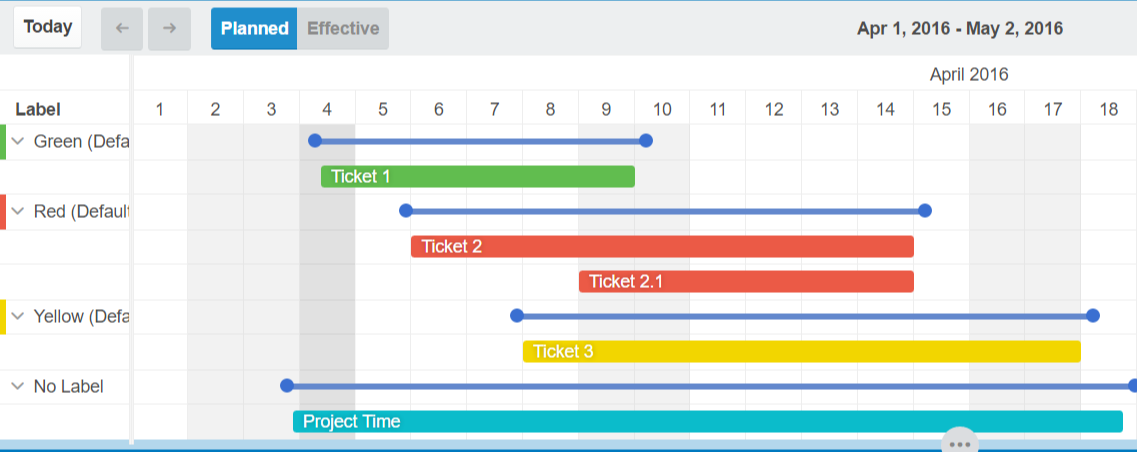
\includegraphics[scale=0.35]{../Images/ticketing-example.png}
			\caption{Esempio di cruscotto Trello}	
		\end{center}
		\end{figure}	
		\item \textbf{Gestione:} nonostante non sia auspicabile è possibile che un evento del genere accada. È essenziale quindi che, attraverso un attento controllo dei tempi di progetto, il responsabile dell'attività comunichi prima della data di scadenza che  il task\addglos sta procedendo a rilento, chiedendo risorse aggiuntive per colmare il ritardo. Se il ritardo fosse incolmabile sarà necessario procedere ad una revisione della pianificazione che permetta di rispettare le scadenze.
		\item \textbf{Riscontro:}
			\begin{itemize}
				\item\textbf{Analisi Iniziale:} il rischio non si è presentato.
				\item\textbf{Progettazione:} il ritardo causato dalla necessità di rivedere i requisiti ha di conseguenza fatto slittare l'inizio delle attività proprie della progettazione, quali la stesura della Specifica Tecnica e Definizione di Prodotto. Essendo il ritardo troppo ampio per partecipare alla RP-max, per mitigarne gli effetti si è deciso di rivedere la pianificazione, come descritto nella \underline{sezione~\ref{Preventivo a finire}} dei Consuntivi, in modo da partecipare alla revisione allo stato RP-min, concentrando quindi l'impegno nella Progettazione Architetturale.
				\item\textbf{Progettazione di dettaglio e codifica:} il rischio non si è presentato.
			\end{itemize}
		\end{itemize}
		\subsubsection{Ritardata partecipazione ad una revisione}							Rappresenta il rischio che per un sommarsi dei problemi sopra elencati il gruppo non possa partecipare ad una revisione nelle date prefissate.
		\begin{itemize}
		\item \textbf{Probabilità:} 1
		\item \textbf{Impatto:} C
		\item \textbf{Controllo:} è compito del Responsabile controllare lo stato del progetto e attuare le adeguate contromisure come riportato nelle precedenti sezioni.
		\item \textbf{Gestione:} tale rischio non è risolvibile, ma obbliga il gruppo a far slittare la propria pianificazione alla data di revisione successiva. Nel caso di un evento così impattante è necessario individuare esattamente i fattori che lo hanno causato e prendere tutte le contromisure necessarie in modo che non possa verificarsi nuovamente alla revisioni successive.
		\item \textbf{Riscontro:}
			\begin{itemize}
				\item\textbf{Analisi Iniziale:} il rischio non si è presentato.
				\item\textbf{Progettazione:} il rischio non si è presentato.
				\item\textbf{Progettazione di dettaglio e codifica:} il rischio si è presentato. Considerando le modifiche da apportare e gli impegni accademici dei membri (ad esempio dare esami per accedere allo stage ) e l'imminente scadenza per la consegna, il gruppo ha deciso di non partecipare alla revisione del 17 giugno. Questa decisione dolorosa ha come conseguenza lo spostamento delle scadenze previste è un'attenta rivalutazione della pianificazione. Il perché di tale ritardo è stato individuato nel sovrapporsi di più impegni, accademici e non, di più elementi del gruppo.
			\end{itemize}
		\end{itemize}
	\pagebreak	
		
	\newpage
	\section{Pianificazione delle risorse}	
	Questa sezione è dedicata all'analisi e distribuzione delle risorse necessarie durante l'intera durata dello sviluppo. Verranno di seguito riportate la scadenze da rispettare per il progetto didattico. Successivamente verranno precisate la suddivisione e rotazione dei ruoli, correlate dal numero di ore dedicato ad ogni attività, nel succedersi delle fasi di sviluppo del progetto. I costi della pianificazione così proposta verranno poi riassunti nel Conto Economico Preventivo.
	\subsection{Scadenze}
	Le Scadenze, cioè le date di revisione, alle quali il gruppo \textbf{Team404} si prefigge di partecipare sono le seguenti:
	\begin{table}[h!]
	\begin{center}
		\begin{tabularx}{240pt}{Xc}
			\textbf{Scadenza} & \textbf{Data}\\
			\midrule
			Revisione dei Requisiti & 18/04/2016\\
			Revisione di Progettazione & 23/05/2016\\
			Revisione di Qualifica & 11/07/2016\\
			Revisione di Accettazione & 24/08/2016\\
			\bottomrule
		\end{tabularx}
	\end{center}
	\caption{Scadenze ufficiali	}
	\end{table}
	
	\subsection{Pianificazione attività di sviluppo}
	Basandosi sulle scadenze riportate si è deciso di suddividere la pianificazione in più parti, ognuna identificata dallo spazio temporale tra un revisione e l'altra. Definita la rotazione dei ruoli, per ogni fase verranno fissate le ore/persona che ognuno dovrà ricoprire nel proprio ruolo.
	 \subsubsection{Rotazione dei ruoli}
I ruoli subiranno una rotazione per permettere a tutti gli elementi di avere esperienza dei vari processi che compongono lo sviluppo di un progetto software complesso. Durante le varie fasi del progetto è possibile, ed auspicabile, che alcuni ruoli non vengano ricoperti da nessun elemento del gruppo, e che un ruolo venga invece ricoperto da più persone. Ad esclusione dell'analisi iniziale, la durata media dei periodi individuati è di un mese; si è quindi deciso di attuare la rotazione dei ruoli circa ogni due settimane, dal momento che una rotazione più dinamica inibirebbe la produttività dei singoli elementi.
		\pagebreak
		\subsubsection{Analisi}
		L'analisi iniziale ha avuto inizio il 20/12/2015 ed è finita il 17/04/2016. Il buon svolgimento di questa fase è prerequisito essenziale per procedere efficientemente alla successiva fase di progettazione. Durante questo periodo il gruppo ha posto la propria attenzione sui seguenti punti:
		\begin{itemize}
		\item Produrre un'attenta analisi dei requisiti che descriva il più fedelmente possibile le esigenze del prodotto;
		\item Stabilire una pianificazione ragionevole delle fasi di progetto;
		\item Definire l'insieme delle norme di progetto e gli obiettivi di qualità da conseguire;
		\item Verificare, correggere e validare il lavoro svolto.
		\end{itemize}
		Le attività sono state svolte secondo rotazione di ruoli riportata in tabella:
		\begin{table}[h!]			
		\begin{center}
			\begin{tabular}{l c c}
			\textbf{Componente} & \textbf{Ruolo I} & \textbf{Ruolo II} \\
			\midrule
			Davide Bortot & Responsabile & Amministratore\\
			Martin Vadice Mbouenda & Amministratore & Analista\\
			Marco Crivellaro & Analista & Verificatore\\
			Alex Beccaro & Analista & Responsabile\\
			Luca Alessio & Analista & Verificatore\\
			Andrea Multineddu & Verificatore & Analista\\
			\midrule
			\end{tabular}
		\end{center}
		\caption{Ruoli Analisi Iniziale}
		\end{table}
		
		La tabelle successive riportano la suddivisione in ore attuata per ogni ruolo e persona:
		\begin{table}[h!]			
		\begin{center}
			\begin{tabular}{l c c c}
			\textbf{Componente} & \textbf{Ore Ruolo I} & \textbf{Ore Ruolo II} & \textbf{Totale Ore}\\
			\midrule
			Davide Bortot & 15 & 8 & 23\\
			Martin Vadice Mbouenda & 17 & 5 & 22\\
			Marco Crivellaro & 15 & 9 & 24 \\
			Alex Beccaro & 19 & 6 & 25\\
			Luca Alessio & 13 & 8 & 21\\
			Andrea Multineddu & 18 & 4 & 22\\
			\midrule
			\textbf{Ore medie per persona} & & & \textbf{22.8}\\
			\end{tabular}
		\end{center}
		\caption{Ore/persona Analisi Iniziale}
		\end{table}
		\begin{table}[h!]			
		\begin{center}
			\begin{tabular}{l c}
			\textbf{Ruolo} & \textbf{Ore Totali} \\
			\midrule
			Analista & 56\\
			Verificatore & 35\\
			Amministratore & 25 \\
			Responsabile & 21\\
			\midrule
			\textbf{Totale} & \textbf{137}\\
			\end{tabular}
		\end{center}
		\caption{Ore/ruolo Analisi Iniziale}
		\end{table}
		\begin{figure}[h!]
		    \centering
			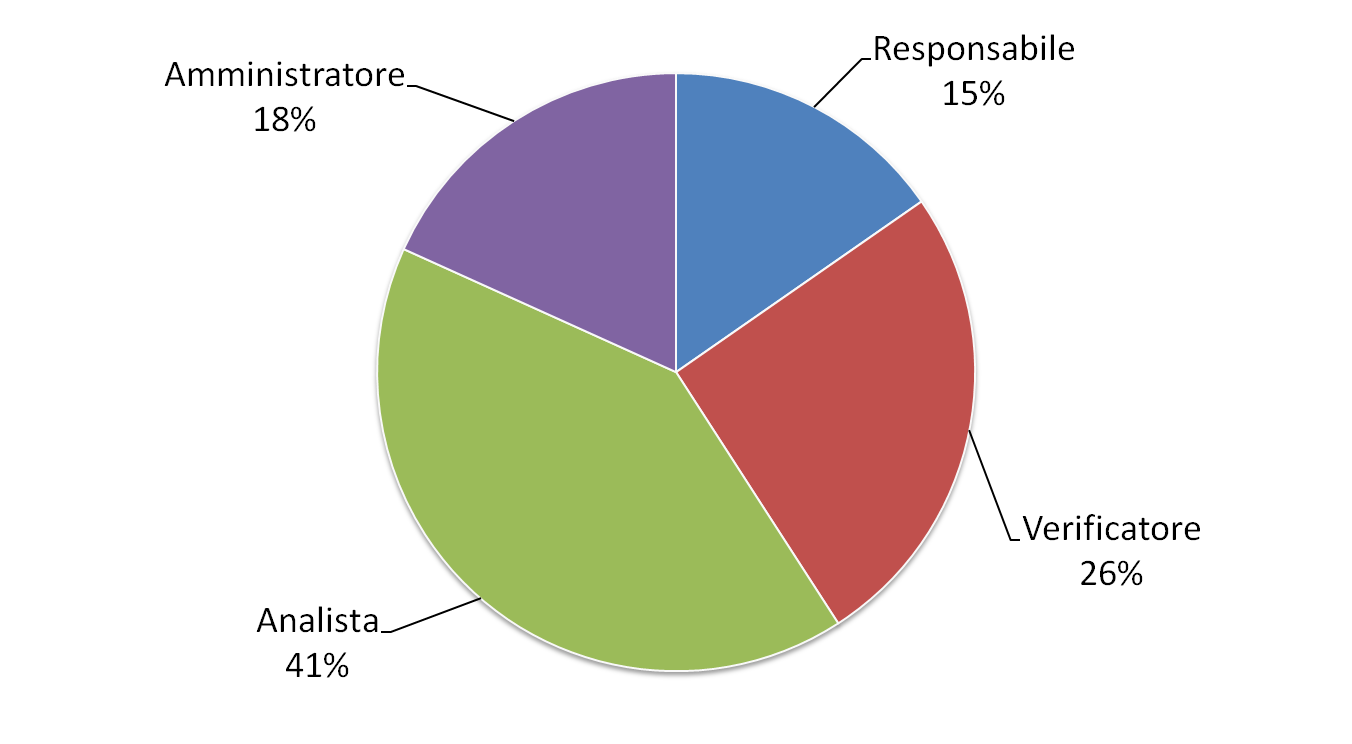
\includegraphics[scale=0.55]{../Images/pie_chart-Analisi_Iniziale}
			\caption{Incisione Ruoli Analisi Iniziale}
		\end{figure}
		
		Come evidenziato dalla Figura 2 la maggior parte dell'impegno è stata riposta nell'assicurare un'approfondita analisi dei requisiti, mentre c'è stato pari impegno nella stesura dei documenti di competenza rispettivamente di Responsabile e Amministratore. Più di un quarto delle ore preventivate è stato usato nel processo di verifica, controllo di qualità e validazione del materiale prodotto, processo che è continuato fino alla data di consegna. I costi sostenuti e le ore svolte in questa prima fase non verranno acclusi al preventivo, ma vengono riportati per completezza.
		\pagebreak
		\subsubsection{Progettazione Architetturale}
		Questa fase ha avuto inizio il 19/04/2016 ed è finita il 22/05/2016. In virtù dell'attenta analisi dei requisiti derivante dalla fase precedente, il gruppo conta di poter iniziare fin da subito un'efficace attività di progettazione. L'uscita dalla fase coinciderà con la partecipazione alla RP-min, quindi alla presentazione dell'architettura del prodotto . In questo periodo lo sviluppo sarà incentrato sui seguenti punti:
		\begin{itemize}
		\item Continuo raffinamento e validazione dei requisiti;
		\item Trasformazione dei requisiti in una solida progettazione architetturale, che costituisca una base il più possibile stabile per futuri incrementi;
		\item Traduzione della progettazione architetturale in progettazione di dettaglio, input concreto per la successiva fase di codifica;
		\item Verificare, correggere e validare il lavoro svolto.
		\end{itemize}
		Le attività si svolgeranno in linea di massima secondo la rotazione di ruoli riportata in Tabella 11. Per garantire a tutti gli elementi di partecipare nel ruolo di progettisti, ruolo principale della fase, alcuni elementi dovranno ricoprire più ruoli contemporaneamente.
		\begin{table}[h!]			
		\begin{center}
			\begin{tabular}{l c c}
			\textbf{Componente} & \textbf{Ruolo I} & \textbf{Ruolo II} \\
			\midrule
			Davide Bortot & Responsabile/Progett & Analista/Ver\\
			Martin Vadice Mbouenda & Analista/Ver & Responsabile/Progett\\
			Marco Crivellaro & Analista/Ver & Progettista\\
			Alex Beccaro & Progettista & Analista/Ver\\
			Luca Alessio & Progettista/Amm & Analista/Ver\\
			Andrea Multineddu & Analista/Ver & Progettista/Amm\\
			\midrule
			\end{tabular}
		\end{center}
		\caption{Ruoli Progettazione}
		\end{table}
		\pagebreak
		
		Le tabelle successive riportano la suddivisione in ore attuata per ogni ruolo e persona:
		\begin{table}[h!]			
		\begin{center}
			\begin{tabular}{l c c c}
			\textbf{Componente} & \textbf{Ore Ruolo I} & \textbf{Ore Ruolo II} & \textbf{Totale Ore}\\
			\midrule
			Davide Bortot & 10/18 & 5/15 & 48\\
			Martin Vadice Mbouenda & 5/14 & 5/18 & 42\\
			Marco Crivellaro & 5/15 & 20 & 40 \\
			Alex Beccaro & 20 & 5/15 & 40\\
			Luca Alessio & 18/5 & 5/15 & 43\\
			Andrea Multineddu & 5/15 & 18/10 & 48\\
			\midrule
			\textbf{Ore medie per persona} & & & \textbf{43,5}\\
			\end{tabular}
		\end{center}
		\caption{Ore/persona Progettazione}
		\end{table}
		\begin{table}[h!]			
		\begin{center}
			\begin{tabular}{l c}
			\textbf{Ruolo} & \textbf{Ore Totali} \\
			\midrule
			Progettista & 112 \\
			Verificatore & 89 \\
			Analista & 30\\
			Amministratore & 15\\
			Responsabile & 15\\
			\midrule
			\textbf{Totale} & \textbf{261}\\
			\end{tabular}
		\end{center}
		\caption{Ore/ruolo Progettazione}
		\end{table}
		\begin{figure}[h!]
		    \centering
			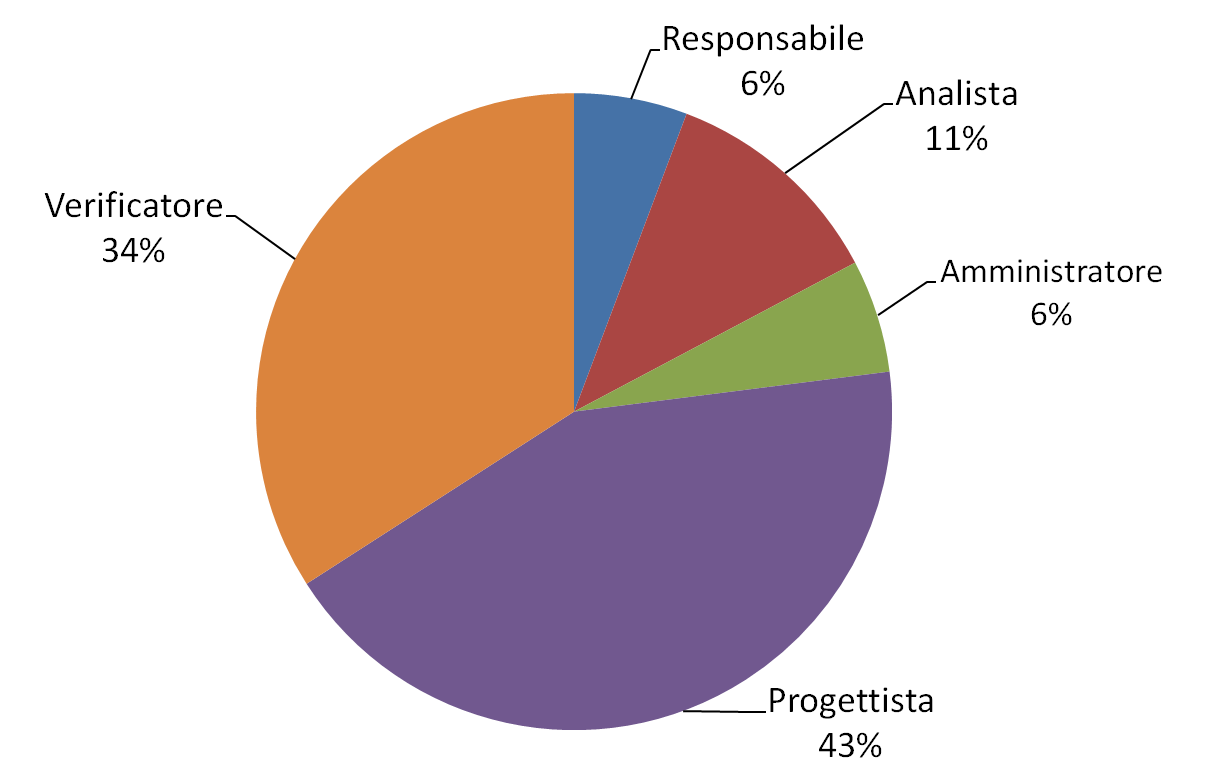
\includegraphics[scale=0.6]{../Images/pie_chart-Progettazione}
			\caption{Incisione Ruoli Progettazione}
		\end{figure}
		
		La suddivisione del lavoro è stata pensata in modo che l'attività del progettista, ruolo che tutti gli elementi ricopriranno almeno una volta durante la fase, sia controllata e supportata da una notevole quantità d'ore dedicate al processo di verifica. Questa è la fase alla quale vengono dedicate più ore in tutto il progetto, in modo da garantire una progettazione completa che permetta di iniziare la codifica senza bisogno di molti aggiustamenti ulteriori.
		\newpage
		\subsubsection{Progettazione di Dettaglio e Codifica}
		Questa fase inizierà il 24/05/2016 e finirà il 10/07/2016. Nel primo periodo vi saranno le ultime attività di perfezionamento e correzione della progettazione; nel contempo inizierà l'attività di codifica basata sulla progettazione di dettaglio prodotta. Come per la fase precedente il processo principale, in questo caso la codifica, sarà continuamente monitorata e validata dal processo di verifica. Nell'ottica di consentire a tutto il gruppo di essere partecipe nel ruolo di Programmatore la rotazione dei ruoli è stata così definita:
		\begin{table}[h!]			
		\begin{center}
			\begin{tabular}{l c c}
			\textbf{Componente} & \textbf{Ruolo I} & \textbf{Ruolo II} \\
			\midrule
			Davide Bortot & Progettista/Ver & Programmatore\\
			Martin Vadice Mbouenda & Programmatore & Progettista/Ver\\
			Marco Crivellaro & Resp/Programm & Verificatore/Amm\\
			Alex Beccaro & Verificatore/Amm & Resp/Programm\\
			Luca Alessio & Programmatore  & Progettista/Ver\\
			Andrea Multineddu & Progettista/Ver & Programmatore\\
			\midrule
			\end{tabular}
		\end{center}
		\caption{Ruoli Codifica}
		\end{table}
		
		Le tabelle successive riportano la suddivisione in ore attuata per ogni ruolo e persona.
		\begin{table}[h!]			
		\begin{center}
			\begin{tabular}{l c c c}
			\textbf{Componente} & \textbf{Ore Ruolo I} & \textbf{Ore Ruolo II} & \textbf{Totale Ore}\\
			\midrule
			Davide Bortot & 5/10 & 20 & 35\\
			Martin Vadice Mbouenda & 18 & 5/10 & 33\\
			Marco Crivellaro & 10/18 & 10/5 & 43 \\
			Alex Beccaro & 10/10 & 5/20 & 45\\
			Luca Alessio & 20 & 10/10 & 40\\
			Andrea Multineddu & 5/10 & 22 & 37\\
			\midrule
			\textbf{Ore medie per persona} & & & \textbf{39}\\
			\end{tabular}
		\end{center}
		\caption{Ore/persona Codifica}
		\end{table}
		\begin{table}[h!]			
		\begin{center}
			\begin{tabular}{l c}
			\textbf{Ruolo} & \textbf{Ore Totali} \\
			\midrule
			Programmatore & 118 \\
			Verificatore & 60\\
			Progettista & 25 \\		
			Responsabile & 15\\
			Amministratore & 15 \\
			\midrule
			\textbf{Totale} & \textbf{233}\\
			\end{tabular}
		\end{center}
		\caption{Ore/ruolo Codifica}
		\end{table}
		
		\begin{figure}[h!]
		    \centering
			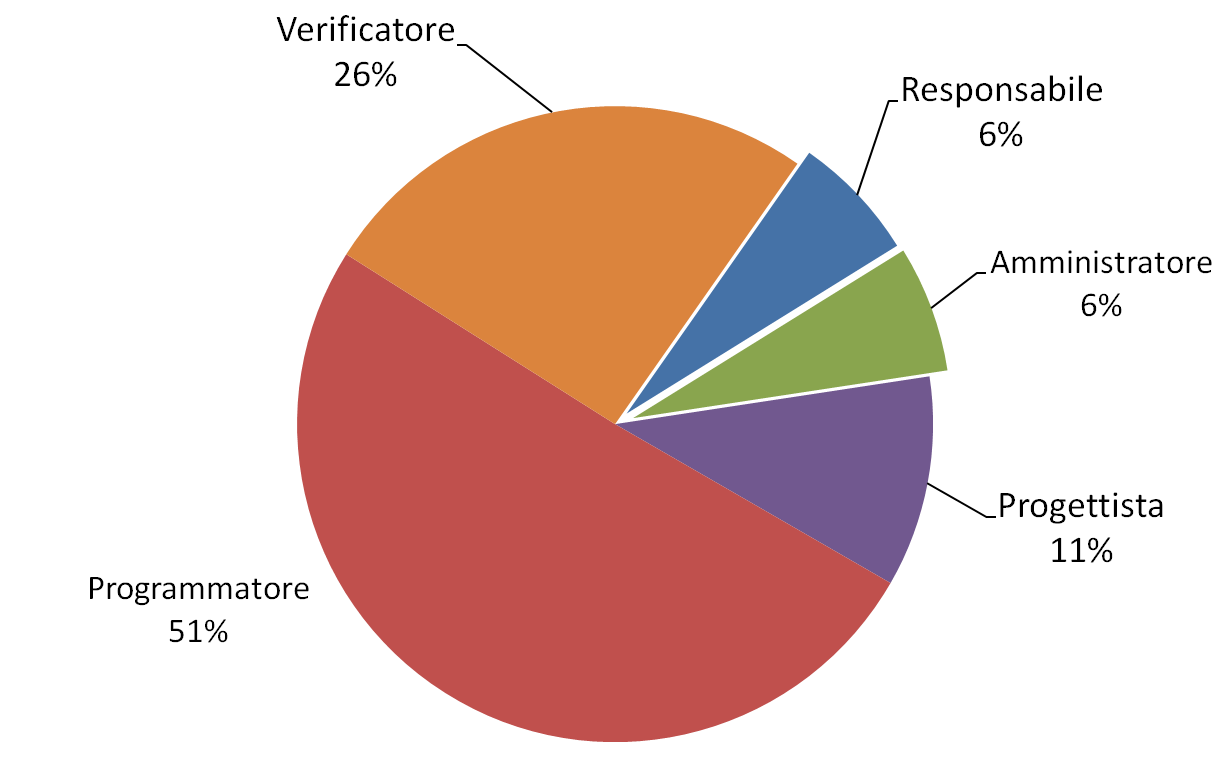
\includegraphics[scale=0.65]{../Images/pie_chart-Codifica}
			\caption{Incisione Ruoli Codifica}
		\end{figure}
		\clearpage
			
		\subsubsection{Verifica e validazione}
		Questa fase inizierà il 12/07/2016 e finirà l' 23/08/2016, in concomitanza con la Revisione di Accettazione. Scopo di quest'ultima fase è procedere ad un'attenta verifica e validazione del software prodotto, integrato in tutte le sue parti, ed al collaudo dell'intero sistema. L'ultima rotazione dei ruoli è stata decisa come in Tabella 17, con l'obiettivo di far partecipe l'intero gruppo del processo di verifica.
		\begin{table}[h!]			
		\begin{center}
			\begin{tabular}{l c c}
			\textbf{Componente} & \textbf{Ruolo I} & \textbf{Ruolo II} \\
			\midrule
			Davide Bortot & Programmatore & Amm/Verificatore\\
			Martin Vadice Mbouenda & Amm/Progettista & Verificatore\\
			Marco Crivellaro & Programmatore & Verificatore\\
			Alex Beccaro & Verificatore & Progettista\\
			Luca Alessio & Verificatore & Resp/Progettista\\
			Andrea Multineddu & Resp/Progettista & Verificatore\\
			\midrule
			\end{tabular}
		\end{center}
		\caption{Ruoli Verifica e Validazione}
		\end{table}
		\begin{table}[h]			
		\begin{center}
			\begin{tabular}{l c c c}
			\textbf{Componente} & \textbf{Ore Ruolo I} & \textbf{Ore Ruolo II} & \textbf{Totale Ore}\\
			\midrule
			Davide Bortot & 5 & 5/10 & 20\\
			Martin Vadice Mbouenda & 10/3 & 10 & 23\\
			Marco Crivellaro & 5 & 15 & 20 \\
			Alex Beccaro & 13 & 5 & 18\\
			Luca Alessio & 5 & 10/5 & 20\\
			Andrea Multineddu & 5/5 & 8 & 18\\
			\midrule
			\textbf{Ore medie per persona} & & & \textbf{20}\\
			\end{tabular}
		\end{center}
		\caption{Ore/persona Verifica e Validazione}
		\end{table}
		
		\begin{table}[h!]			
		\begin{center}
			\begin{tabular}{l c}
			\textbf{Ruolo} & \textbf{Ore Totali} \\
			\midrule
			Verificatore & 61\\
			Programmatore & 15 \\
			Progettista & 13 \\
			Amministratore & 15 \\
			Responsabile & 15\\
			\midrule
			\textbf{Totale} & \textbf{119}\\
			\end{tabular}
		\end{center}
		\caption{Ore/ruolo Verifica e Validazione}
		\end{table}
		
		\begin{figure}[h!]
		    \centering
			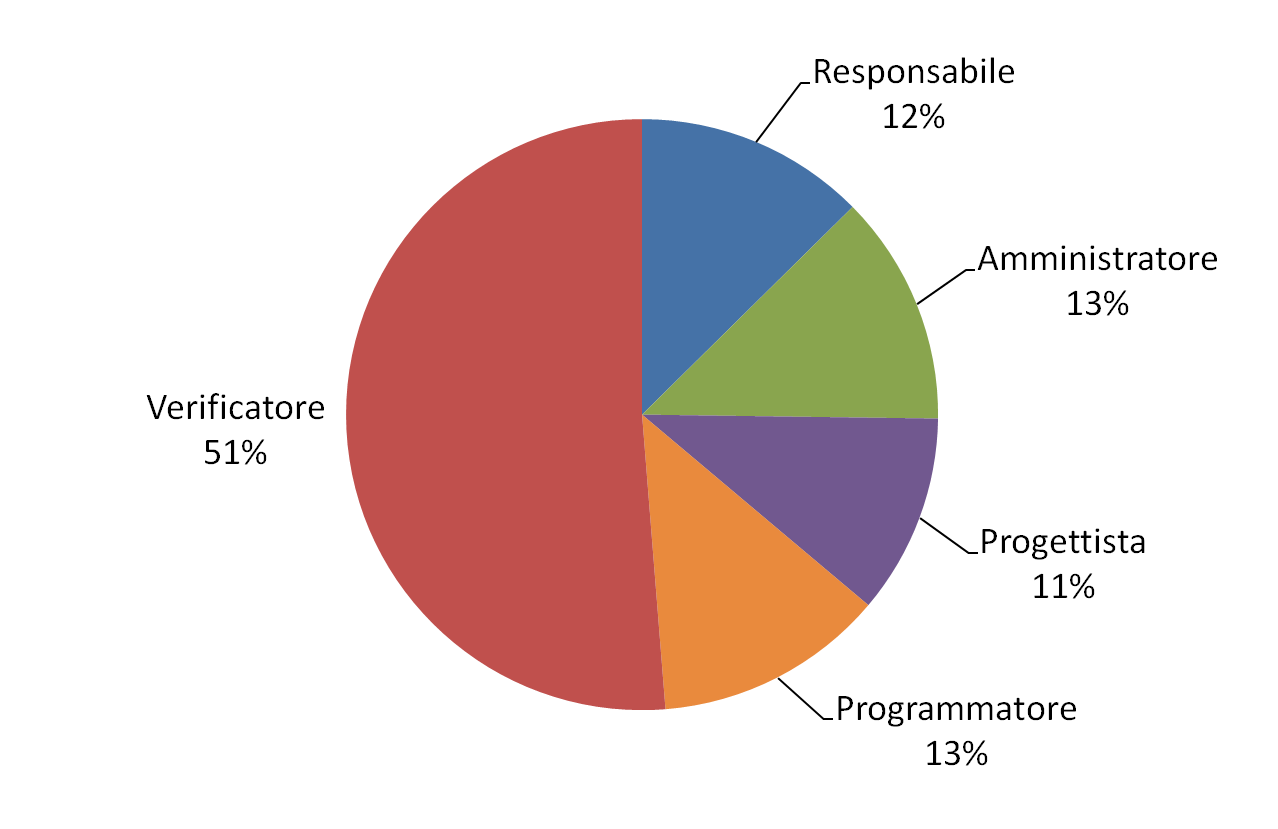
\includegraphics[scale=0.6]{../Images/pie_chart-V&V}
			\caption{Incisione Ruoli Verifica e Validazione}
		\end{figure}
		
	\newpage
	\section{Conto Economico Preventivo}
	\subsection{Vincoli economici e didattici}
	Come da regolamento del progetto didattico il costo minimo preventivato non dev'essere inferiore a 13.000,00 \euro. Tuttavia tale cifra è calcolata basandosi su gruppi di progetto composti da 7 persone; essendo il nostro organico composto di soli 6 elementi, è logico abbassare percentualmente il tetto minimo per adeguarlo alle ore/lavoro a nostra disposizione, ottenendo un costo preventivo minimo di 11.142 \euro. Tale preventivo va calcolato sulla base dei costi orari per ruolo riportati nella seguente tabella.

	\begin{table}[h!]
	\begin{center}
		\begin{tabularx}{150pt}{Xc}
			\textbf{Ruolo} & \textbf{\euro/ora}\\
			\midrule
			Responsabile & 30 \\
			Analista & 25 \\
			Amministratore & 20 \\
			Progettista & 22 \\
			Programmatore & 15 \\
			Verificatore & 15 \\
			\midrule
		\end{tabularx}
		\end{center}
	\caption{Costi orari per ruolo}
	\end{table}
	
La pianificazione deve inoltre assicurare un'equa distribuzione del carico di lavoro individuale (le ore d'impegno pro persona devono situarsi tra un minimo di 85 e un massimo di 105) e la rotazione dei ruoli tra gli elementi del gruppo.
	\subsection{Preventivo}
	Sulla base dei costi in Tabella 19 e della suddivisione del lavoro definita nel Capitolo 6 il costo stimato per lo sviluppo del progetto è di seguito riportato.
	\begin{table}[h!]
	\begin{center}
		\begin{tabular}{l c c}
			\textbf{Ruolo} & \textbf{Ore} & \textbf{Costo}\\
			\midrule
			Responsabile & 45 & 1 350\\
			Analista & 30 & 750\\
			Amministratore & 45 & 900\\
			Progettista & 150 & 3 300\\
			Programmatore & 133 & 1 995\\
			Verificatore & 210 & 3 150\\
			\midrule
			\textbf{Totale} & \textbf{613} & \textbf{11 445}
		\end{tabular}
		\end{center}
	\caption{Preventivo}
	\end{table}
	
	Risulta evidente che la maggior parte dei costi è improntata a sostenere una solida attività di progettazione ed un continuo processo di verifica e validazione. Il preventivo proposto presenta un surplus di \textbf{303 \euro} rispetto al preventivo minimo di 11 142 \euro.
	\subsubsection{Incidenza Fasi}
	 Procedendo con un'analisi più fine, vengono presentati i costi relativi alle singole fasi del progetto, che evidenziano ulteriormente come l'attività nella quale verrà posto il maggior sforzo sia quella di Progettazione. I costi divisi per fase sono riassunti nella tabella successiva.
	\begin{table}[h!]
	\begin{center}
		\begin{tabular}{l c c}
			\textbf{Fase di Progetto} & \textbf{Ore} & \textbf{Costo}\\
			\midrule
			Progettazione & 261 & 5 299 \\
			Codifica & 236 & 3 970 \\
			Verifica e Validazione & 119 & 2 176\\
			\midrule
			\textbf{Totale} & \textbf{613} & \textbf{11 445}
		\end{tabular} 
		\end{center}
	\caption{Costi per Fase}
	\end{table}
	\begin{figure}[h!]
		\centering
		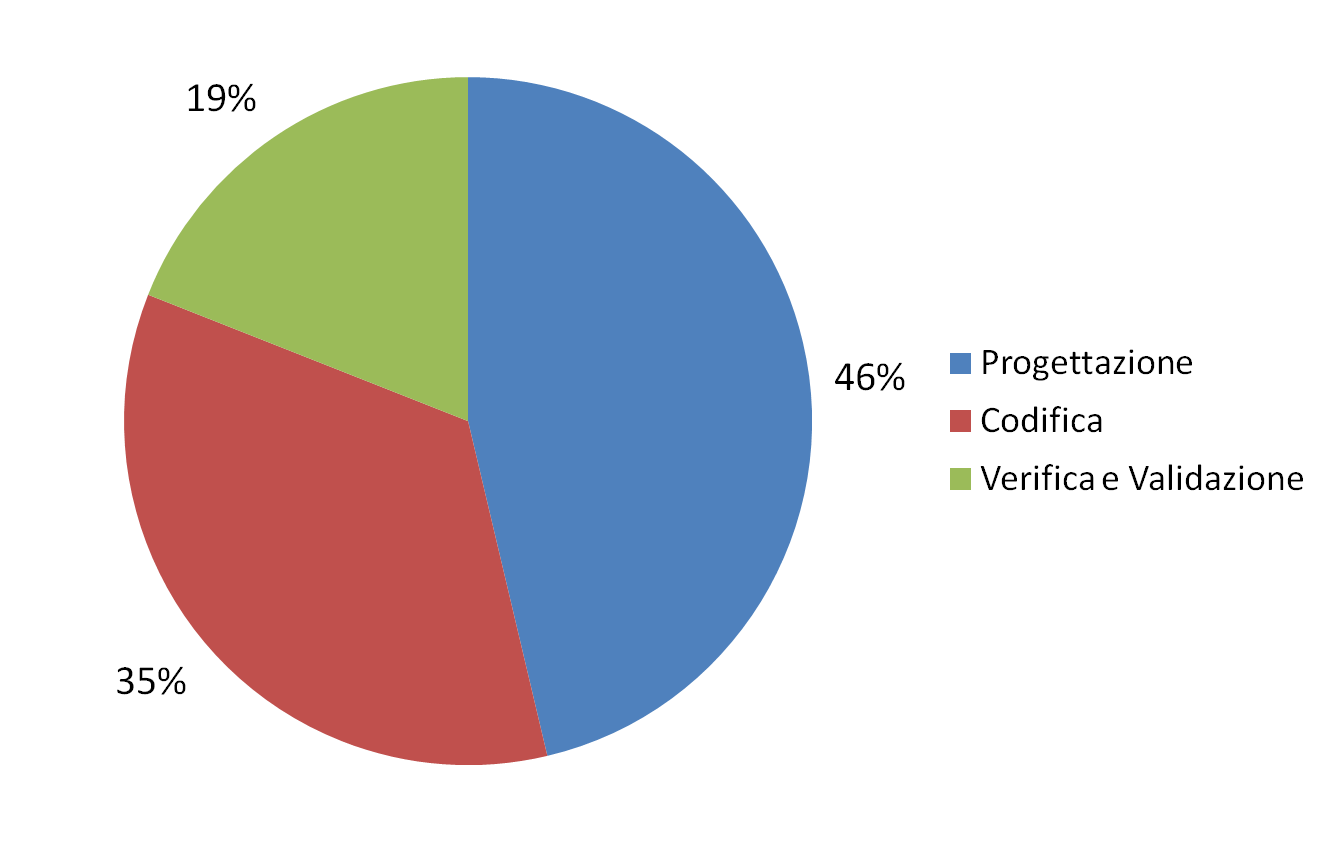
\includegraphics[scale=0.6]{../Images/pie_chart-Preventivo_Fasi}
		\caption{Incidenza Fasi di progetto}
	\end{figure}
	\pagebreak
	\subsubsection{Incidenza Ruoli}
	La figura seguente riassume velocemente il peso di ciascun ruolo riguardo la durata dell'intero progetto. Le attività di spicco sono la progettazione e la verifica.
	\begin{figure}[h!]
		\centering
		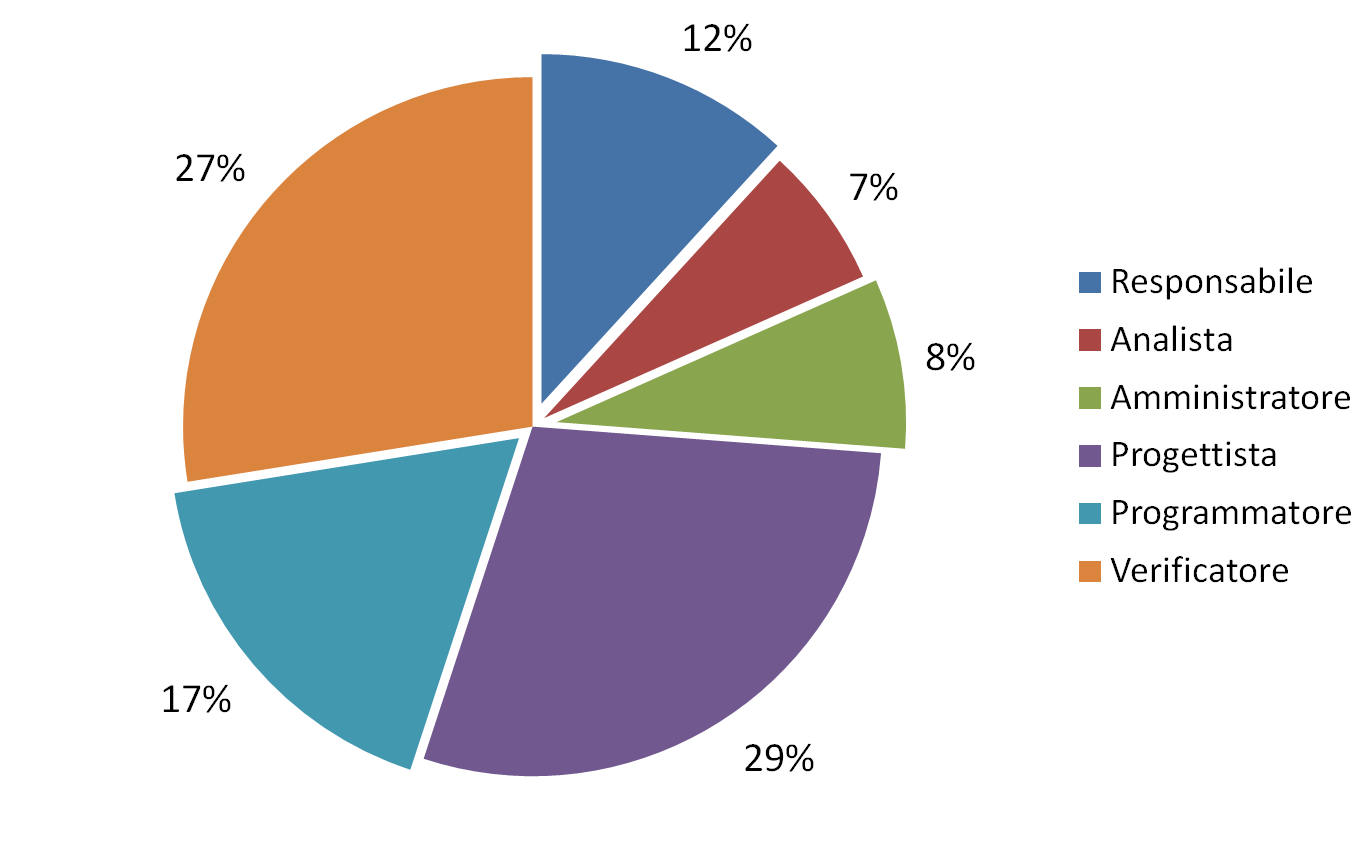
\includegraphics[scale=0.6]{../Images/pie_chart-Preventivo_Ruoli}
		\caption{Incidenza Ruoli nel progetto}
	\end{figure}
	\newpage
	\subsection{Prospetto Orario}
	Secondo quanto riportato nella sezione Vincoli, le ore di lavoro per persona devono situarsi tra un minimo di 85 e un massimo di 105. Il prospetto orario che rispecchia la pianificazione precedentemente presentata è il seguente:
	\begin{table}[h!]
		\hspace{0.6cm}\begin{tabular}{l c c c c c c}
		 	& \textbf{Davide} & \textbf{Martin} & \textbf{Marco} & \textbf{Alex} & \textbf{Luca} & \textbf{Andrea}\\
			 & \textbf{Bortot} & \textbf{V.Mbouenda} & \textbf{Crivellaro} & \textbf{Beccaro} & \textbf{Alessio} & \textbf{Multineddu}\\
			\midrule
			Responsabile 	& 10 & 5  & 10  & 5  & 10 & 5 \\
			Analista 		& 5  & 5  & 5   & 5  & 5  & 5 \\
			Amministratore 	& 5  & 10 & 5   & 10 & 5  & 10\\
			Progettista 	& 23 & 26 & 20  & 25 & 28 & 28\\
			Programmatore 	& 25 & 18 & 23  & 20 & 25 & 22\\
			Verificatore 	& 35 & 34 & 40  & 38 & 30 & 33\\
			\midrule
			\textbf{Totale} & \textbf{103} & \textbf{98} & \textbf{103} & \textbf{103} & \textbf{103} & \textbf{103}
		\end{tabular}
	\caption{Prospetto Orario}
	\end{table}
	
	Si è deciso di assegnare qualche ora di lavoro in meno a Martin Vadice Mbouenda, che è studente lavoratore e, in quanto tale, è normale possa dedicare meno tempo al presente progetto.
	\newpage
		
	\section{Consuntivi} \label{conto:consuntivo}
	\subsection{Fase di Analisi}
	Viene proposto di seguito il consuntivo relativo alla fase di Analisi con l'obiettivo di rilevare le discrepanze tra la pianificazione e le ore effettuate, e le tendenze che ne derivano. Seguirà un preventivo a finire basato sui precedenti risultati.
	\newline
	Il grafico a barre seguente illustra il rapporto tra ore di lavoro pianificate e ore effettuate per ruolo.
	\begin{figure}[h!]
		\centering
		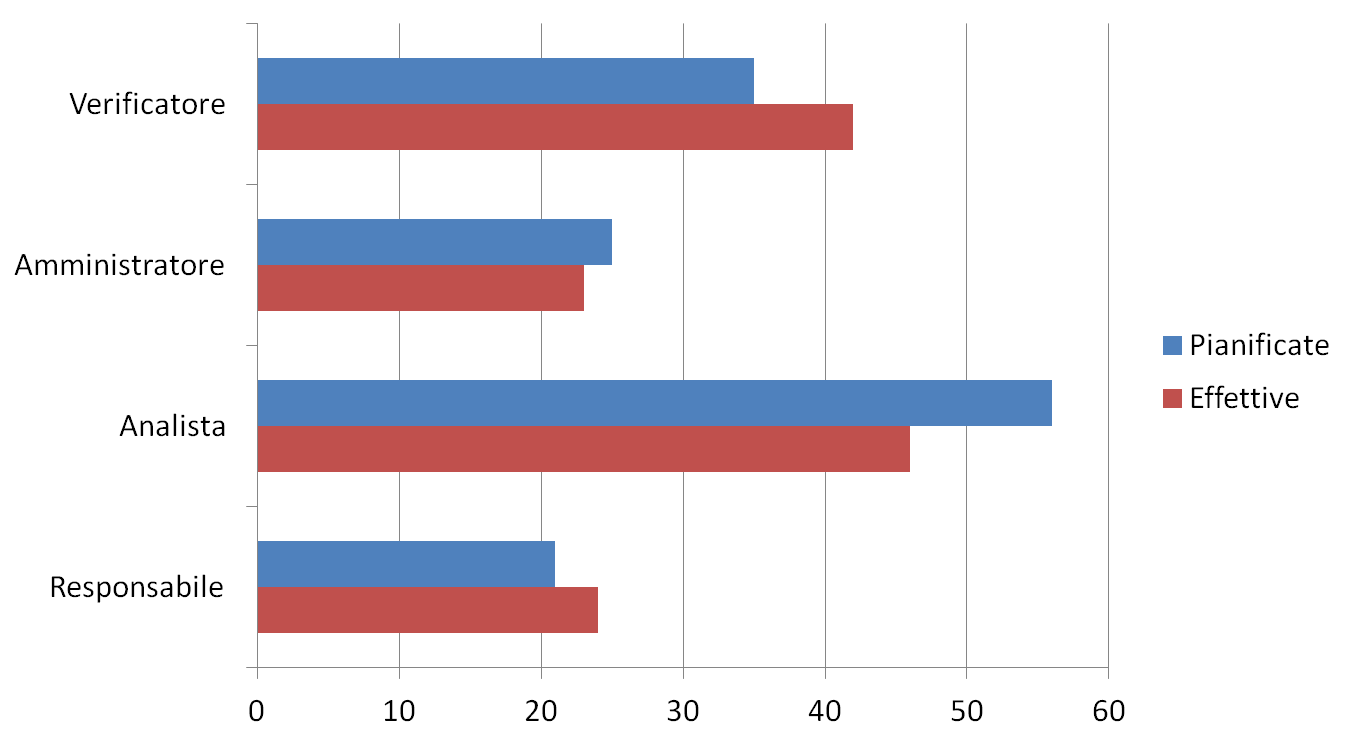
\includegraphics[scale=0.7]{../Images/chart-Consuntivo_Ore_Analisi}
	\caption{Consuntivo Ore Analisi}
	\end{figure}
	
	\begin{table}[h!]
	\begin{center}
		\begin{tabular}{l c c c}
			\textbf{Ruolo} & \textbf{Preventivo} & \textbf{Consuntivo} &\textbf{Bilancio}\\
			\midrule
			Responsabile 	& 630 	& 720	& +90	\\
			Analista 		& 1400 	& 1150	& -250	\\
			Amministratore 	& 500 	& 460	& -40	\\
			Verificatore 	& 525 	& 630	& +105	\\
			\midrule
			\textbf{Totale} & \textbf{3055 \euro} & \textbf{2960 \euro}	& \textbf{-95 \euro}
		\end{tabular}
		\end{center}
	\caption{Consuntivo Costi Analisi}
	\end{table}

	La fase si è conclusa con un costo di \textbf{2960 \euro}, inferiore di \textbf{95 \euro} rispetto a quanto preventivato.
	
	\subsubsection{Consuntivo di periodo}
	Dal confronto tra consuntivo e preventivo risulta in modo evidente una sottostima delle ore dedicate al ruolo di verificatore e una sovrastima delle ore dedicate agli analisti; i due errori di stima hanno di fatto pareggiato il costo consuntivo, che non si discosta di molto da quanto preventivato. Durante questo periodo il gruppo ha lavorato con diligenza rispettando i tempi di consegna; è degno di nota che l'assegnazione di specifici task corredati da deadline adeguate ha impatto particolarmente positivo sulla produttività del gruppo. \newline
	Il minor numero di ore utilizzate effettivamente per il ruolo di "Analista" potrebbe far pensare che l'analisi dei requisiti prodotta fosse sufficientemente corposa. Le correzioni successive alla Revisione dei Requisiti e l'incontro col proponente riportato nel verbale \emph{"Verbale\_Esterno-2016-04-22"} hanno dimostrato invece che l'attività di analisi e categorizzazione dei requisiti necessiterà di ulteriore impegno; a tal riguardo sono state applicate le correzioni riportate nel preventivo a finire.
	\subsubsection{Preventivo a finire}
	\label{Preventivo a finire}
	La sottostima delle ore di verifica ha portato a rivalutare la pianificazione presentata in sede di Revisione dei Requisiti. In particolare sono state ripartite le ore di verifica delle fasi di Progettazione e Codifica in favore di una distribuzione più equa che assesta l'impegno della verifica a circa un terzo dell'impegno totale per ogni periodo. La sovrastima delle ore di analisi, unita alle considerazioni della sezione precedente, ha portato ad un ulteriore rivisitazione della pianificazione che comprendesse più ore per il ruolo di "Analista" durante i medesimi periodi.
	Viene di seguito presentata la pianificazione rivisitata per i periodi soggetti e il preventivo a finire calcolato sulla nuova pianificazione, dove col colore rosso vengono evidenziati i cambiamenti tra le due versioni. La nuova pianificazione tiene anche conto del riscontro dei rischi dalla fase di Analisi iniziale fino ai primi giorni del periodo di Progettazione, che ha portato a rivalutare la scelta di partecipare alla RP-max. Il gruppo parteciperà alla RP-min, quindi le attività della progettazione verranno suddivise in due: la Progettazione Architetturale e la Progettazione di Dettaglio; la seconda andrà ad aggiungersi al periodo che nel preventivo precedente veniva denominato "Codifica".
	
	\subsubsubsection{Progettazione Architetturale}	
	\begin{table}[h!]			
		\begin{center}
			\begin{tabular}{l c c}
			\textbf{Componente} & \textbf{Ruolo I} & \textbf{Ruolo II} \\
			\midrule
			Davide Bortot & Responsabile/Progett & Analista/Ver\\
			Martin Vadice Mbouenda & Analista/Ver & Responsabile/Progett\\
			Marco Crivellaro & Analista/Ver & Progettista\\
			Alex Beccaro & Progettista & Analista/Ver\\
			Luca Alessio & Progettista/Amm & Analista/Ver\\
			Andrea Multineddu & Analista/Ver & Progettista/Amm\\
			\midrule
			\end{tabular}
		\end{center}
		\caption{Ruoli Progettazione Architetturale}
		\end{table}

		\begin{table}[h!]			
		\begin{center}
			\begin{tabular}{l l l l}
			\textbf{Componente} & \textbf{Ore Ruolo I} & \textbf{Ore Ruolo II} & \textbf{Totale Ore}\\
			\midrule
			Davide Bortot & 10/12\textcolor{red}{(-6)} & 7\textcolor{red}{(+2)}/10\textcolor{red}{(-5)} & 39\textcolor{red}{(-9)}\\
			Martin Vadice Mbouenda & 7\textcolor{red}{(+2)}/14 & 5/11\textcolor{red}{(-7)} & 37\textcolor{red}{(-5)}\\
			Marco Crivellaro & 7\textcolor{red}{(+2)}/13\textcolor{red}{(-2)} & 14\textcolor{red}{(-6)} & 34\textcolor{red}{(-6)}\\
			Alex Beccaro & 14\textcolor{red}{(-6)} & 7\textcolor{red}{(+2)}/13\textcolor{red}{(-2)} & 34\textcolor{red}{(-6)}\\
			Luca Alessio & 12\textcolor{red}{(-6)}/5 & 6\textcolor{red}{(+1)}/11\textcolor{red}{(-4)} & 34\textcolor{red}{(-9)}\\
			Andrea Multineddu & 7\textcolor{red}{(+2)}/13\textcolor{red}{(-2)} & 12\textcolor{red}{(-6)}/10 & 42\textcolor{red}{(-6)}\\
			\midrule
			\textbf{Ore medie per persona} & & & \textbf{36,6}\\
			\end{tabular}
		\end{center}
		\caption{Ore/persona Progettazione Architetturale}
		\end{table}
		\begin{table}[h!]			
		\begin{center}
			\begin{tabular}{l l l}
			\textbf{Ruolo} & \textbf{Ore Totali} & \textbf{Costi} \\
			\midrule
			Progettista & 75\textcolor{red}{(-37)} & 1650\textcolor{red}{(-814)}\\
			Verificatore & 74\textcolor{red}{(-15)} & 1110\textcolor{red}{(-225)}\\
			Analista & 41\textcolor{red}{(+11)} & 1025\textcolor{red}{(+275)}\\
			Amministratore & 15 & 300\\
			Responsabile & 15 & 450\\
			\midrule
			\textbf{Totale} & \textbf{220}\textcolor{red}{(-41)} & \textbf{4535 \euro}\textcolor{red}{(-764\euro)}\\
			\end{tabular}
		\end{center}
		\caption{Ore e Costi Progettazione Architetturale}
		\end{table}
		\begin{figure}[h!]
		    \centering
			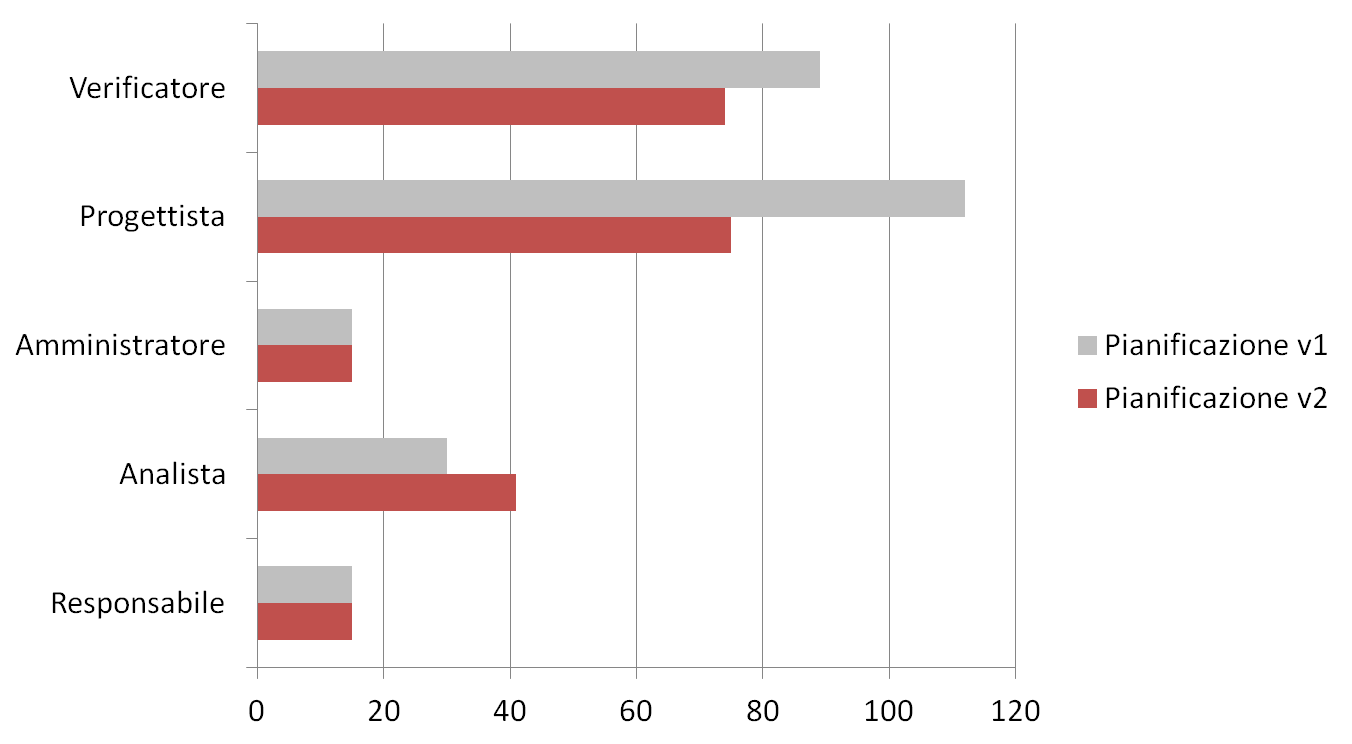
\includegraphics[scale=0.7]{../Images/chart-Confronto_Pianificazioni1vs2_Progettazione.png}
			\caption{Confronto Ore Pianificazione v1 e Pianificazione v2 per la Progettazione}
		\end{figure}	
		\clearpage
		
		\subsubsubsection{Progettazione di Dettaglio e Codifica}
		\begin{table}[h!]			
		\begin{center}
			\begin{tabular}{l c c}
			\textbf{Componente} & \textbf{Ruolo I} & \textbf{Ruolo II} \\
			\midrule
			Davide Bortot & Progettista/Ver & Programmatore\\
			Martin Vadice Mbouenda & Programm/\textcolor{red}{Analista} & \textcolor{red}{Progettista}/Ver\\
			Marco Crivellaro & Resp/Programm & Verificatore/Amm\\
			Alex Beccaro & Verificatore/Amm & Resp/Programm\\
			Luca Alessio & Programm/\textcolor{red}{Analista} & Progettista/Ver\\
			Andrea Multineddu & Progettista/Ver & Programmatore\\
			\midrule
			\end{tabular}
		\end{center}
		\caption{Ruoli Progettazione di Dettaglio e Codifica}
		\end{table}
		
		\begin{table}[h!]			
		\begin{center}
			\begin{tabular}{l l l l}
			\textbf{Componente} & \textbf{Ore Ruolo I} & \textbf{Ore Ruolo II} & \textbf{Totale Ore}\\
			\midrule
			Davide Bortot & 11\textcolor{red}{(+6)}/16\textcolor{red}{(+6)} & 18\textcolor{red}{(-2)} & 45\textcolor{red}{(+10)}\\
			Martin Vadice Mbouenda & 15\textcolor{red}{(-3)}/6\textcolor{red}{(+6)} & 6\textcolor{red}{(+1)}/13\textcolor{red}{(+3)} & 40\textcolor{red}{(+7)}\\
			Marco Crivellaro & 10/17\textcolor{red}{(-1)} & 18\textcolor{red}{(+8)}/5 & 50\textcolor{red}{(+7)} \\
			Alex Beccaro & 16\textcolor{red}{(+6)}/10 & 5/21\textcolor{red}{(+1)} & 52\textcolor{red}{(+7)}\\
			Luca Alessio & 15\textcolor{red}{(-5)}/6\textcolor{red}{(+6)} & 16\textcolor{red}{(+6)}/13\textcolor{red}{(+3)} & 50\textcolor{red}{(+10)}\\
			Andrea Multineddu & 11\textcolor{red}{(+6)}/15\textcolor{red}{(+5)} & 18\textcolor{red}{(-4)} & 44\textcolor{red}{(+7)}\\
			\midrule
			\textbf{Ore medie per persona} & & & \textbf{46,8}\\
			\end{tabular}
		\end{center}
		\caption{Ore/persona Progettazione di Dettaglio e Codifica}
		\end{table}
		\begin{table}[h!]			
		\begin{center}
			\begin{tabular}{l l l}
			\textbf{Ruolo} & \textbf{Ore Totali} & \textbf{Costi}\\
			\midrule
			Programmatore & 104\textcolor{red}{(-14)} & 1560\textcolor{red}{(-210)} \\
			Verificatore & 91\textcolor{red}{(+31)} & 1365\textcolor{red}{(+465)}\\
			Progettista & 44\textcolor{red}{(+19)} & 968\textcolor{red}{(+418)}\\
			Analista & 12\textcolor{red}{(+12)} & 300\textcolor{red}{(+300)}\\		
			Responsabile & 15 & 450\\
			Amministratore & 15 & 300\\
			\midrule
			\textbf{Totale} & \textbf{281}\textcolor{red}{(+48)} & \textbf{4943 \euro}\textcolor{red}{(+973\euro)}\\
			\end{tabular}
		\end{center}
		\caption{Ore e Costi Progettazione di Dettaglio e Codifica}
		\end{table}
		\clearpage
		
		\begin{figure}[h!]
		    \centering
			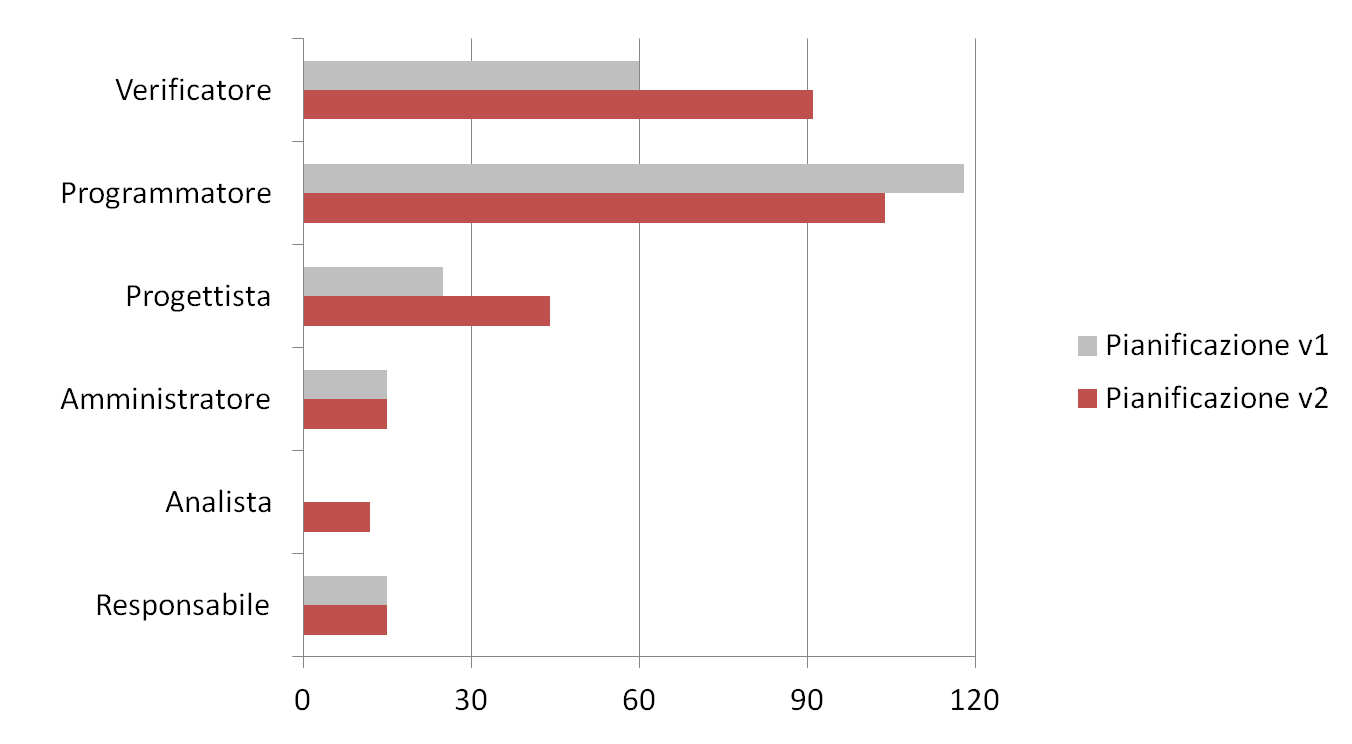
\includegraphics[scale=0.7]{../Images/chart-Confronto_Pianificazioni1vs2_Codifica.png}
			\caption{Confronto Ore Pianificazione v1 e Pianificazione v2 per la Codifica}
		\end{figure}		
		
		\subsubsubsection{Prospetto Orario Aggiornato}
		\begin{table}[h!]
		\hspace{0.2cm}\begin{tabular}{l l l l l l l}
		 	& \textbf{Davide} & \textbf{Martin} & \textbf{Marco} & \textbf{Alex} & \textbf{Luca} & \textbf{Andrea}\\
			 & \textbf{Bortot} & \textbf{Mbouenda} & \textbf{Crivellaro} & \textbf{Beccaro} & \textbf{Alessio} & \textbf{Multineddu}\\
			\midrule
			Responsabile 	& 10 & 5  & 10  & 5  & 10 & 5 \\
			Analista 		& 7\textcolor{red}{(+2)}  & 13\textcolor{red}{(+8)}  & 7\textcolor{red}{(+2)}   & 7\textcolor{red}{(+2)}  & 12\textcolor{red}{(+7)}  & 7\textcolor{red}{(+2)} \\
			Amministratore 	& 5  & 10 & 5   & 10 & 5  & 10\\
			Progettista 	& 23 & 20\textcolor{red}{(-6)} & 14\textcolor{red}{(-6)}  & 19\textcolor{red}{(-6)} & 28 & 28\\
			Programmatore 	& 23\textcolor{red}{(-2)} & 15\textcolor{red}{(-3)} & 22\textcolor{red}{(-1)}  & 21\textcolor{red}{(+1)} & 20\textcolor{red}{(-5)} & 18\textcolor{red}{(-4)}\\
			Verificatore 	& 36\textcolor{red}{(+1)} & 37\textcolor{red}{(+3)} & 46\textcolor{red}{(+6)}  & 42\textcolor{red}{(+4)} & 29\textcolor{red}{(-1)} & 36\textcolor{red}{(+3)}\\
			\midrule
			\textbf{Totale} & \textbf{104}\textcolor{red}{(+1)} & \textbf{100}\textcolor{red}{(+2)} & \textbf{104}\textcolor{red}{(+1)} & \textbf{104}\textcolor{red}{(+1)} & \textbf{104}\textcolor{red}{(+1)} & \textbf{104}\textcolor{red}{(+1)}
		\end{tabular}
	\caption{Prospetto Orario v2}
	\end{table}	
	\clearpage	
		
		\subsubsubsection{Preventivo}
		Il preventivo a finire basato sulle precedenti modifiche è il seguente
		
		\begin{table}[h!]
		\begin{center}
			\begin{tabular}{l l l}
			\textbf{Ruolo} & \textbf{Ore} & \textbf{Costo}\\
			\midrule
				Responsabile & 45 & 1 350\\
				Analista & 53\textcolor{red}{(+23)} & 1 325 \textcolor{red}{(+575)}\\
				Amministratore & 45 & 900\\
				Progettista & 132\textcolor{red}{(-18)} & 2 904 \textcolor{red}{(-396)}\\
				Programmatore & 119\textcolor{red}{(-14)} & 1 785 \textcolor{red}{(-210)}\\
				Verificatore & 226\textcolor{red}{(+16)} & 3 390 \textcolor{red}{(+240)}\\
			\midrule
			\textbf{Totale} & \textbf{620}\textcolor{red}{(+7)} & \textbf{11 654 \euro}\textcolor{red}{(+209\euro)}
			\end{tabular}
		\end{center}
			\caption{Preventivo a finire}
		\end{table}
	\noindent
	Il preventivo a finire si discosta dal preventivo precedente con una maggiorazione di \textbf{209 \euro}, inevitabile con l'aumento delle ore del ruolo di "Analista". Col procedere del progetto e con i successivi consuntivi si valuterà se il budget aggiunto sarà utilizzato e se sarà possibile produrre un preventivo a finire che risparmi costi aggiuntivi. L'impegno per singola persona rimane comunque entro i limiti prefissati (non più di 105 ore). Seguono  le differenze di costo divise per periodo.
	\begin{table}[h!]
	\begin{center}
		\begin{tabular}{l l l}
			\textbf{Periodo di Progetto} & \textbf{Ore} & \textbf{Costo}\\
			\midrule
			Progettazione Architetturale & 220\textcolor{red}{(-41)} & 4 535\textcolor{red}{(+118)} \\
			Prog. di Dettaglio e Codifica & 281\textcolor{red}{(+48)} & 4 943\textcolor{red}{(+155)} \\
			Verifica e Validazione & 119 & 2 176\\
			\midrule
			\textbf{Totale} & \textbf{620}\textcolor{red}{(+7)} & \textbf{11 654 \euro}\textcolor{red}{(+209\euro)}
		\end{tabular} 
		\end{center}
	\caption{Costi per periodo preventivo a finire}
	\end{table}	
	
	Con la suddivisione delle attività di progettazione anche il rispettivo impegno è stato diviso e ridistribuito. Ora il periodo più corposo, sia per ore preventivate che per costi, è il periodo di Progettazione di Dettaglio e Codifica. Eventuali aggiustamenti alla pianificazione e al preventivo dei periodi di progetto rimanenti verranno valutati con il calcolo del prossimo consuntivo e controllando dinamicamente il livello dei rischi.
	
	\newpage
	
	\subsection{Fase di Progettazione Architetturale}
	Viene proposto di seguito il consuntivo relativo alla fase di Progettazione Architetturale. Il grafico a barre seguente illustra il rapporto tra ore di lavoro pianificate e ore effettuate per
ruolo. 	
	
	\begin{figure}[h!]
		\centering
		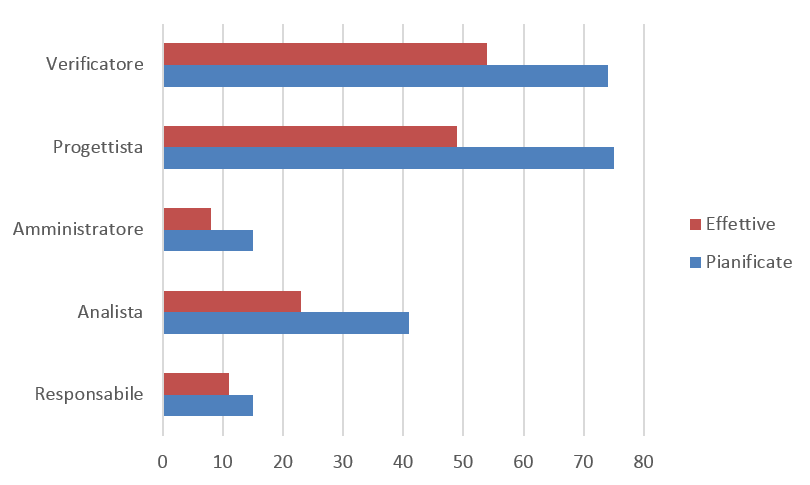
\includegraphics[scale=0.7]{../Images/chart-Consuntivo_Ore_Progettazione}
	\caption{Consuntivo Ore Progettazione Architetturale}
	\end{figure}
	
	\begin{table}[h!]
	\begin{center}
		\begin{tabular}{l c c c}
			\textbf{Ruolo} & \textbf{Preventivo} & \textbf{Consuntivo} &\textbf{Bilancio}\\
			\midrule
			Responsabile 	& 450 	& 330	& -120	\\
			Analista 		& 1025 	& 575	& -450	\\
			Amministratore 	& 300 	& 160	& -140	\\			
			Progettista 	& 1650 	& 1078	& -572	\\
			Verificatore 	& 1110 	& 810	& -300	\\
			\midrule
			\textbf{Totale} & \textbf{4535 \euro} & \textbf{2953 \euro}	& \textbf{-1582 \euro}
		\end{tabular}
		\end{center}
	\caption{Consuntivo Costi Progettazione Architetturale}
	\end{table}
	
La fase si è conclusa con un costo di \textbf{2953 \euro}, inferiore di \textbf{1582 \euro} rispetto a quanto preventivato.
	\subsubsection{Consuntivo di periodo}
	In questo periodo, si osserva una grande differenza tra il costo preventivato e il costo effettivo. 
	  Questo è dovuto principalmente alla scelta di andare non in RP-max\addglos ma in RP-min\addglos, il che ci a portato spostare una fetta di ore di questa fase alla prossima per fronteggiare la progettazione di dettaglio. Durante questo periodo il gruppo ha lavorato con maggior precisione e collaborazione, provvedendo a verifiche continue lungo il periodo in modo da tenere tutti i lavori allineati con gli obbiettivi fissati.  
	
	
	\subsubsection{Preventivo a finire}
		La maggior considerazione dell'impegno necessario per la progettazione di dettaglio ci ha portato a una nuova rivalutazione della pianificazione in modo da ricollocare nell'ordine di un terzo, parte del tempo preventivato per questa fase nella successiva.
	\subsubsubsection{Progettazione di Dettaglio e Codifica}
		\begin{table}[h!]			
		\begin{center}
			\begin{tabular}{l c c}
			\textbf{Componente} & \textbf{Ruolo I} & \textbf{Ruolo II} \\
			\midrule
			Davide Bortot & Progettista/Ver & Programmatore\\
			Martin Vadice Mbouenda & Programm/Analista & Progettista/Ver\\
			Marco Crivellaro & Resp/Programm & Verificatore/Amm\\
			Alex Beccaro & Verificatore/Amm & Resp/Programm\\
			Luca Alessio & Programm/Analista & Progettista/Ver\\
			Andrea Multineddu & Progettista/Ver & Programmatore\\
			\midrule
			\end{tabular}
		\end{center}
		\caption{Ruoli Progettazione di Dettaglio e Codifica}
		\end{table}
		
		\begin{table}[h!]			
		\begin{center}
			\begin{tabular}{l l l l}
			\textbf{Componente} & \textbf{Ore Ruolo I} & \textbf{Ore Ruolo II} & \textbf{Totale Ore}\\
			\midrule
			Davide Bortot & 19\textcolor{red}{(+8)}/16 & 21\textcolor{red}{(+3)} & 56\textcolor{red}{(+11)}\\
			Martin Vadice Mbouenda & 17\textcolor{red}{(+2)}/9\textcolor{red}{(+3)} & 15\textcolor{red}{(+9)}/14\textcolor{red}{(+1)} & 55\textcolor{red}{(+15)}\\
			Marco Crivellaro & 10/24\textcolor{red}{(-7)} & 24\textcolor{red}{(+6)}/5 & 63\textcolor{red}{(+13)} \\
			Alex Beccaro & 25\textcolor{red}{(+9)}/10 & 5/24\textcolor{red}{(+3)} & 64\textcolor{red}{(+12)}\\
			Luca Alessio & 18\textcolor{red}{(+3)}/9\textcolor{red}{(+3)} & 17\textcolor{red}{(+1)}/15\textcolor{red}{(+2)} & 59\textcolor{red}{(+9)}\\
			Andrea Multineddu & 17\textcolor{red}{(+6)}/20\textcolor{red}{(+5)} & 18/4\textcolor{red}{(+4)} & 59\textcolor{red}{(+15)}\\
			\midrule
			\textbf{Ore medie per persona} & & & \textbf{59,3\textcolor{red}{(+12,5)}}\\
			\end{tabular}
		\end{center}
		\caption{Ore/persona Progettazione di Dettaglio e Codifica}
		\end{table}
		\begin{table}[h!]			
		\begin{center}
			\begin{tabular}{l l l}
			\textbf{Ruolo} & \textbf{Ore Totali} & \textbf{Costi}\\
			\midrule
			Programmatore & 122\textcolor{red}{(+18)} & 1830\textcolor{red}{(+270)} \\
			Verificatore & 114\textcolor{red}{(+16)} & 1710\textcolor{red}{(+345)}\\
			Progettista & 68\textcolor{red}{(+22)} & 1496\textcolor{red}{(+528)}\\
			Analista & 22\textcolor{red}{(+19)} & 550\textcolor{red}{(+250)}\\		
			Responsabile & 15 & 450 \\
			Amministratore & 15 & 300 \\
			\midrule
			\textbf{Totale} & \textbf{356}\textcolor{red}{(+75)} & \textbf{6336 \euro}\textcolor{red}{(+1393\euro)}\\
			\end{tabular}
		\end{center}
		\caption{Ore e Costi Progettazione di Dettaglio e Codifica}
		\end{table}
		\clearpage
		
		\begin{figure}[h!]
		    \centering
			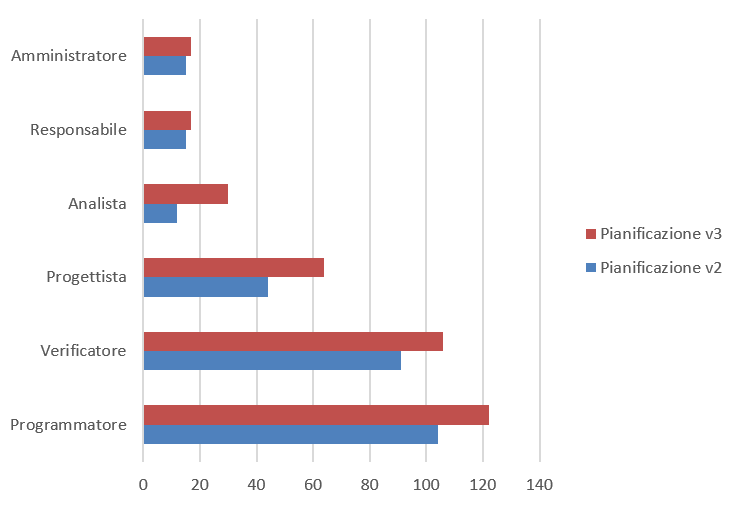
\includegraphics[scale=0.7]{../Images/chart-Confronto_Pianificazioni2vs3_Progettazione.png}
			\caption{Confronto Ore Pianificazione v2 e Pianificazione v3 per la Codifica}
		\end{figure}		
		
	\subsubsubsection{Prospetto Orario Aggiornato}
		\begin{table}[h!]
		\hspace{0.2cm}\begin{tabular}{l l l l l l l}
		 	& \textbf{Davide} & \textbf{Martin} & \textbf{Marco} & \textbf{Alex} & \textbf{Luca} & \textbf{Andrea}\\
			 & \textbf{Bortot} & \textbf{Mbouenda} & \textbf{Crivellaro} & \textbf{Beccaro} & \textbf{Alessio} & \textbf{Multineddu}\\
			\midrule
			Responsabile 	& 8\textcolor{red}{(-2)} & 3\textcolor{red}{(-2)}  & 10  & 5  & 10 & 5 \\
			Analista 		& 4\textcolor{red}{(-3)}  & 12\textcolor{red}{(-1)}  & 4\textcolor{red}{(-3)}   & 4\textcolor{red}{(-3)}  & 13\textcolor{red}{(+1)}  & 8\textcolor{red}{(+1)} \\
			Amministratore 	& 5  & 10 & 5   & 10 & 3\textcolor{red}{(-2)}  & 5\textcolor{red}{(-5)}\\
			Progettista 	& 27\textcolor{red}{(+4)} & 24\textcolor{red}{(+4)} & 8\textcolor{red}{(-6)}  & 15\textcolor{red}{(-4)} & 26\textcolor{red}{(-2)} & 30\textcolor{red}{(+2)}\\
			Programmatore 	& 26\textcolor{red}{(+3)} & 17\textcolor{red}{(+2)} & 29\textcolor{red}{(+7)}  & 24\textcolor{red}{(+3)} & 23\textcolor{red}{(+3)} & 18\\
			Verificatore 	& 34\textcolor{red}{(-2)} & 34\textcolor{red}{(-3)} & 48\textcolor{red}{(+2)}  & 46\textcolor{red}{(+4)} & 29 & 38\textcolor{red}{(+2)}\\
			\midrule
			\textbf{Totale} & \textbf{104} & \textbf{100} & \textbf{104} & \textbf{104} & \textbf{104} & \textbf{104}
		\end{tabular}
	\caption{Prospetto Orario v3}
	\end{table}	
	\clearpage	
	
	\subsubsubsection{Preventivo}
		Il preventivo a finire basato sulle precedenti modifiche è il seguente
		
		\begin{table}[h!]
		\begin{center}
			\begin{tabular}{l l l}
			\textbf{Ruolo} & \textbf{Ore} & \textbf{Costo}\\
			\midrule
				Responsabile & 41\textcolor{red}{(-4)} & 1 230\\
				Analista & 45\textcolor{red}{(-8)} & 1 125 \textcolor{red}{(+575)}\\
				Amministratore & 38\textcolor{red}{(+7)} & 760\\
				Progettista & 130\textcolor{red}{(-2)} & 2 860 \textcolor{red}{(-396)}\\
				Programmatore & 137\textcolor{red}{(+18)} & 2 055 \textcolor{red}{(-210)}\\
				Verificatore & 229\textcolor{red}{(+3)} & 3 435 \textcolor{red}{(+240)}\\
			\midrule
			\textbf{Totale} & \textbf{620} & \textbf{11 435 \euro}\textcolor{red}{(-219\euro)}
			\end{tabular}
		\end{center}
			\caption{Preventivo a finire}
		\end{table}
		
		Il preventivo a finire si discosta dal preventivo precedente con una differenza di \textbf{189\euro} dovuto alla scelta di andare alla RP-min\addglos. Parte delle ore previste per la progettazione architetturale è  stata ricollocato esclusivamente nella prossima fase per fare fronte alla progettazione di dettaglio, mantenendo l'impegno per per ogni componente del gruppo sotto la soglia massima di 105 ore. Seguono le differenze di costo divise per periodo.
		
		\begin{table}[h!]
	\begin{center}
		\begin{tabular}{l l l}
			\textbf{Periodo di Progetto} & \textbf{Ore} & \textbf{Costo}\\
			\midrule
			Progettazione Architetturale & 145\textcolor{red}{(-75)} & 2 953\textcolor{red}{(-1582)} \\
			Prog. di Dettaglio e Codifica & 356\textcolor{red}{(+75)} & 6 336\textcolor{red}{(+1393)} \\
			Verifica e Validazione & 119 & 2 176\\
			\midrule
			\textbf{Totale} & \textbf{620} & \textbf{11 465\euro}\textcolor{red}{(-189\euro)}
		\end{tabular} 
		\end{center}
	\caption{Costi per periodo preventivo a finire}
	\end{table}	
		
		Dalle tabelle precedente, si nota che le ore effettivamente svolte sono inferiore a quelle preventivate, soprattutto per via dello spostamento di ore della progettazione di dettaglio, ma anche grazie alla migliore collaborazione del team e a un uso migliore degli strumento di documentazione e di sviluppo da parte del gruppo. Il tutto ci ha permesso di risparmiare tempo senza incidere sul raggiungimento degli obbiettivi prefissati. Nonostante ciò, l'importo totale effettivo rimane superiore di \textbf{323\euro}.
	
		\newpage
	
		\subsection{Fase di Progettazione di Dettaglio e Codifica}
	Viene proposto di seguito il consuntivo relativo alla fase di Progettazione di Dettaglio e di codifica. Il grafico a barre seguente illustra il rapporto tra ore di lavoro pianificate e ore effettuate per ruolo. 	
	
	\begin{figure}[h!]
		\centering
		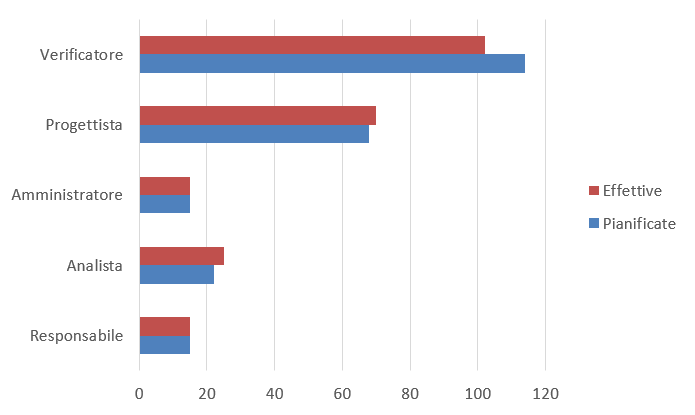
\includegraphics[scale=0.7]{../Images/chart-Consuntivo_Ore_Prog_Det_Cod}
	\caption{Consuntivo Ore Progettazione di Dettaglio}
	\end{figure}
	
	\begin{table}[h!]
	\begin{center}
		\begin{tabular}{l c c c}
			\textbf{Ruolo} & \textbf{Preventivo} & \textbf{Consuntivo} &\textbf{Bilancio}\\
			\midrule 
			Responsabile 	& 450 	& 450	& 0		\\
			Analista 		& 550 	& 625	& 75	\\
			Amministratore 	& 300 	& 300	& 0		\\			
			Progettista 	& 1496 	& 1540	& 44 	\\
			Verificatore 	& 1710 	& 1545	& -165	\\
			Programmatore	& 1830	& 1575  & -255	\\
			\midrule
			\textbf{Totale} & \textbf{6336 \euro} & \textbf{ 6035 \euro}	& \textbf{ -301\euro}
		\end{tabular}
		\end{center}
	\caption{Consuntivo Costi Progettazione di dettaglio e Codifica}
	\end{table}
	
La fase si è conclusa con un costo di \textbf{ 6035 \euro}, inferiore di \textbf{ 301 \euro} rispetto a quanto preventivato.
	\subsubsection{Consuntivo di periodo} \label{con:consuper}
	Avendo saltato una revisione, abbiamo dilazionato il lavoro su un arco temporale più ampio e questo ci ha permesso di lavorare in modo più sereno alla progettazione di dettaglio migliorando l'efficienza e risparmiando così un po' di tempo.  
	 		
	\subsubsection{Preventivo a finire} \label{con:prevfinire}
		La maggior considerazione dell'impegno necessario per la progettazione di dettaglio ci ha portato a una nuova rivalutazione della pianificazione in modo da ricollocare, nell'ordine di un terzo, il tempo preventivato per questa fase nella successiva.
	\subsubsubsection{Verifica e validazione}
		\begin{table}[h!]			
		\begin{center}
			\begin{tabular}{l r r r c}
\textbf{Componente} & \textbf{Ruolo I (ore)}&\textbf{Ruolo II (ore)}&\textbf{Ruolo III (ore)}&\textbf{Totale Ore}\\
			\midrule
			Davide Bortot 		& Amministratore(5)		&Programmatore(6) 	&Verificatore(10) 	& 21\\			
			Martin V. Mbouenda  & Progettista(3)		&Verifica)(16)		& Amministratore(6)& 25	\\
			Marco Crivellaro 	& Programmatore(9)	 	& Verificatore(15)	&					& 24	\\
			Alex Beccaro 		& Verificatore(15)		& Progettista(5)	&					& 20	\\
			Luca Alessio 		&Responsabile(10)		& Programmatore(6) 	& Verificatore(6)	& 22	\\
			Andrea Multineddu 	& Progettista(5)		&Verificatore(10)	& Responsabile(5)	& 20	\\
			\midrule
			\textbf{Ore medie per persona} & & & &\textbf{19.83}\\
			\end{tabular}
		\end{center}
		\caption{Ruoli Verifica e validazione}
		\end{table}
		

		\begin{table}[h!]			
		\begin{center}
			\begin{tabular}{l l l}
			\textbf{Ruolo} & \textbf{Ore Totali} & \textbf{Costi}\\
			\midrule
			Programmatore 	& 21 	& 225 	\euro	\\
			Verificatore 	& 72 	& 915	\euro	\\
			Progettista 	& 13 	& 286	\euro	\\		
			Responsabile 	& 15 	& 450 	\euro	\\
			Amministratore 	& 11 	& 300 	\euro	\\
			\midrule
			\textbf{Totale} & \textbf{132} & \textbf{ 2176 \euro}\\
			\end{tabular}
		\end{center}
		\caption{Ore e Costi Verifica e validazione}
		\end{table}
		\clearpage
		
		\begin{figure}[h!]
		    \centering
			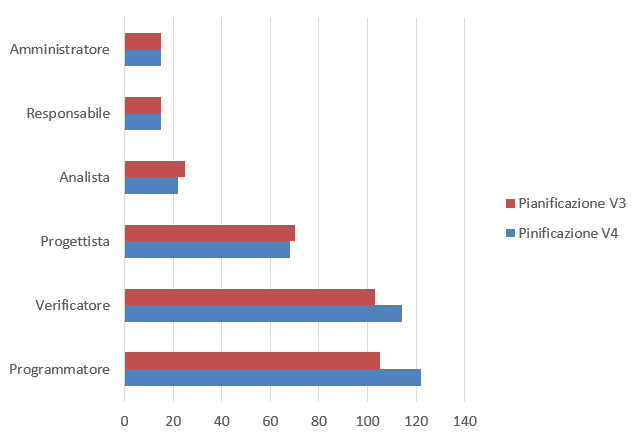
\includegraphics[scale=0.7]{../Images/chart-Confronto_Progettazione3vs4_Codifica.png}
			\caption{Confronto Ore Pianificazione v3 e Pianificazione v4 per la Codifica}
		\end{figure}		
		
	\subsubsubsection{Prospetto Orario Aggiornato}
		\begin{table}[h!]
		\hspace{0.2cm}\begin{tabular}{l c c c c c c}
& \textbf{Davide} & \textbf{Martin}   & \textbf{Marco} 		& \textbf{Alex}    & \textbf{Luca}    & \textbf{Andrea}\\
& \textbf{Bortot} & \textbf{Mbouenda} & \textbf{Crivellaro} & \textbf{Beccaro} & \textbf{Alessio} &\textbf{Multineddu}\\
			\midrule
			Responsabile 	& 8 	& 3  	& 10 	& 5 	& 10 	& 5 \\
			Analista 		& 4  	& 12  	& 11  	& 4 	& 13  	& 4 \\
			Amministratore 	& 5  	& 6 	& 5   	& 10 	& 3  	& 5	\\
			Progettista 	& 27 	& 26 	& 8  	& 15 	& 27 	& 29	\\
			Programmatore 	& 24 	& 17 	& 24  	& 21 	& 20 	& 20\\
			Verificatore 	& 36 	& 35 	& 44  	& 45 	& 30 	& 39\\
			\midrule
			\textbf{Totale} & \textbf{104} & \textbf{99} & \textbf{102} & \textbf{100} & \textbf{103} & \textbf{102}
		\end{tabular}
	\caption{Prospetto Orario v4}
	\end{table}	
	\clearpage	
	
	\subsubsubsection{Preventivo}
		Il preventivo a finire basato sulle precedenti modifiche è il seguente
		
		\begin{table}[h!]
		\begin{center}
			\begin{tabular}{l r r}
			\textbf{Ruolo} 		& \textbf{Ore} 	& \textbf{Costo}\\
			\midrule
				Responsabile 	& 41 			& 1 230\euro		\\
				Analista 		& 48 			& 1 200\euro 	\\
				Amministratore 	& 34 			& 680\euro		\\
				Progettista 	& 132 			& 2 904\euro 	\\
				Programmatore 	& 126 			& 1 890\euro		\\
				Verificatore 	& 229 			& 3 435\euro		\\
			\midrule
			\textbf{Totale} 	& \textbf{610} 	& \textbf{ 11 339 \euro}
			\end{tabular}
		\end{center}
			\caption{Preventivo a finire}
		\end{table}
		
		Il preventivo a finire si discosta leggermente dal preventivo precedente con una differenza di \textbf{96\euro}; l'ampio arco temporale a disposizione, avendo saltato la precedente scadenza, ci ha permesso di organizzarci meglio e di rispettare le ore preventivate ad inizio progetto.
		
		\begin{table}[h!]
	\begin{center}
		\begin{tabular}{l l l}
			\textbf{Periodo di Progetto} 	& \textbf{Ore} 	& \textbf{Costo}\\
			\midrule
			Progettazione Architetturale	& 145 			& 2 953 \\
			Prog. di Dettaglio e Codifica 	& 333 			& 6 035 \\
			Verifica e Validazione 			& 132 			& 2 351	\\
			\midrule
			\textbf{Totale} 				&\textbf{610} 	&\textbf{11 339\euro}
		\end{tabular} 
		\end{center}
	\caption{Costi per periodo preventivo a finire}
	\end{table}	
		
		Dalle tabelle precedenti, si nota che le ore effettivamente svolte sono inferiori a quelle preventivate, soprattutto per via di una migliore collaborazione del team e a un uso migliore degli strumenti di documentazione e di sviluppo da parte del gruppo. Il tutto ci ha permesso di risparmiare tempo senza incidere sul raggiungimento degli obbiettivi prefissati. Questa fase si conclude con preventivo a finire inferiore di \textbf{106\euro} rispetto al preventivo iniziale.
	
			
\end{document}	